\documentclass[11pt,]{article}
\usepackage[]{mathpazo}
\usepackage{amssymb,amsmath}
\usepackage{subcaption}
\usepackage{ifxetex,ifluatex}
\usepackage{fixltx2e} % provides \textsubscript
\ifnum 0\ifxetex 1\fi\ifluatex 1\fi=0 % if pdftex
  \usepackage[T1]{fontenc}
  \usepackage[utf8]{inputenc}
\else % if luatex or xelatex
  \ifxetex
    \usepackage{mathspec}
  \else
    \usepackage{fontspec}
  \fi
  \defaultfontfeatures{Ligatures=TeX,Scale=MatchLowercase}
\fi
% use upquote if available, for straight quotes in verbatim environments
\IfFileExists{upquote.sty}{\usepackage{upquote}}{}
% use microtype if available
\IfFileExists{microtype.sty}{%
\usepackage{microtype}
\UseMicrotypeSet[protrusion]{basicmath} % disable protrusion for tt fonts
}{}
\usepackage[margin=1in]{geometry}
\usepackage{hyperref}
\hypersetup{unicode=true,
            pdftitle={Milestone 6},
            pdfborder={0 0 0},
            breaklinks=true}
\urlstyle{same}  % don't use monospace font for urls
\usepackage{natbib}
\bibliographystyle{plainnat}
\usepackage{graphicx,grffile}
\makeatletter
\def\maxwidth{\ifdim\Gin@nat@width>\linewidth\linewidth\else\Gin@nat@width\fi}
\def\maxheight{\ifdim\Gin@nat@height>\textheight\textheight\else\Gin@nat@height\fi}
\makeatother
% Scale images if necessary, so that they will not overflow the page
% margins by default, and it is still possible to overwrite the defaults
% using explicit options in \includegraphics[width, height, ...]{}
\setkeys{Gin}{width=\maxwidth,height=\maxheight,keepaspectratio}
\IfFileExists{parskip.sty}{%
\usepackage{parskip}
}{% else
\setlength{\parindent}{0pt}
\setlength{\parskip}{6pt plus 2pt minus 1pt}
}
\setlength{\emergencystretch}{3em}  % prevent overfull lines
\providecommand{\tightlist}{%
  \setlength{\itemsep}{0pt}\setlength{\parskip}{0pt}}
\setcounter{secnumdepth}{5}
% Redefines (sub)paragraphs to behave more like sections
\ifx\paragraph\undefined\else
\let\oldparagraph\paragraph
\renewcommand{\paragraph}[1]{\oldparagraph{#1}\mbox{}}
\fi
\ifx\subparagraph\undefined\else
\let\oldsubparagraph\subparagraph
\renewcommand{\subparagraph}[1]{\oldsubparagraph{#1}\mbox{}}
\fi

%%% Use protect on footnotes to avoid problems with footnotes in titles
\let\rmarkdownfootnote\footnote%
\def\footnote{\protect\rmarkdownfootnote}


\usepackage[below]{placeins}

\begin{document}
\begin{titlepage}
  \centering
    
\includegraphics[width=\linewidth]{ms6-figures/logo} % also works with logo.pdf
    \linespread{1.2}\Large{Mapping the Risk of International Infectious Disease Spread
    (MRIIDS)}

   \linespread{1.2}\large{A project funded through USAID’s ``Combating Zika and
     Future Threats: A Grand Challenge for Development'' program}
   \vfill
    Milestone 6: Increased complexity of the simple model to include data from Milestone 5.
    \vfill
  \end{titlepage}
\tableofcontents

\newpage

\begin{figure}
   \centering
   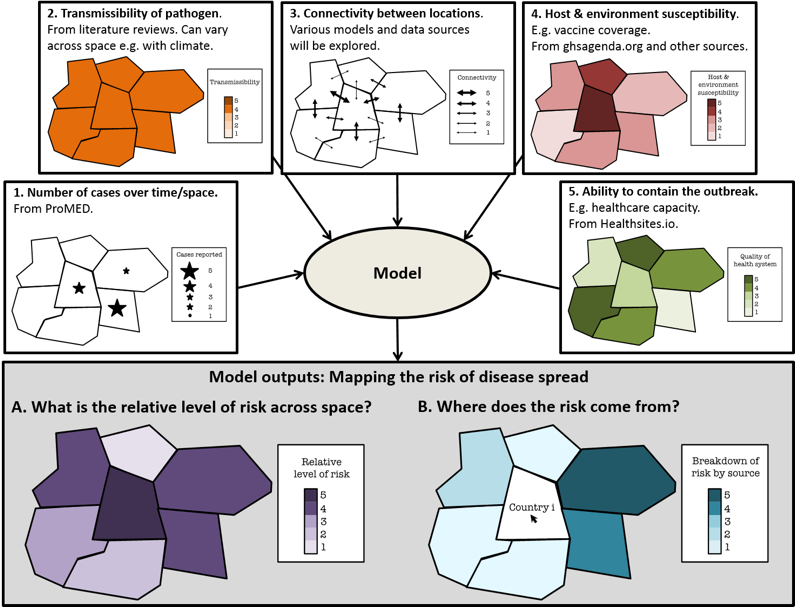
\includegraphics[]{ms6-figures/schematic}
  \caption{Schematic of the Project}
\end{figure}

\section{Milestone Description}\label{milestone-description}

Increased complexity of the simple model to include data from Milestone
5. Automated testing and validating procedures implemented where
possible. Explore procedures for multiple models comparison and accounting for
uncertainty.

\section{Overview}

In Milestone 4, we presented a simple transmission model that made use of
historical case counts (data stream 1), information about the
transmissibility of the pathogen (data stream 2) and geographical
characterization (data stream 3) to predict future risk. 
In this approach, the geographical characterization was not fully integrated in the model:
first transmissibility was estimated from case count data, then future incidence was predicted, and 
finally, the predicted incidence was distributed geographically according to the spatial distribution 
and population density of each geographical unit.

To achieve the goals outlined in Milestone 6, we built on the model presented in Milestone 4 
(ML4) to integrate geographical information into our inference procedure.
Having achieved this, other characteristics defined at the geographical
scale of reference such as the health care capacity of a location, can be 
added to the model.

In essence, by integrating the spatial information into the inference
and prediction phases, we have developed a complex model that has the potential to
account for the multiple data streams initially described.

Therefore, our new complex model has the ability to:
\begin{itemize}
\item estimate model parameters: including parameters linked to geographical spread (or
potentially health care capacity,
\item predict the regional/international spread of Ebola, relying on those parameters' estimates. 
\end{itemize}

We have also established the procedure for the validation process
using historical data and are exploring various possibilities for multi-model comparison. 

For the model validation, we rely on both ProMED/HealthMap incidence data, which are 
at the national scale, and WHO reported data which are at the district level. The advantage 
of using the more spatially refined WHO data is that it allows increased statistical power to 
infer the spatial parameters of the model (i.e. more movements occur at finer spatial scale, 
therefore the `signature' of movement in incidence data is more identifiable at finer scale).
This exercise could be viewed as:
\begin{itemize}
\item demonstrating the flexible nature of our framework, i.e. 
the model is designed to be flexible in term of the choice of spatial scale, and
\item a proof of concept to argue that reporting spatially refined incidence count can improve our ability to
predict spatial spread.
\end{itemize}

\section{Presentation of the model}\label{sec:model}

The number of cases at a location \(j\) at time \(t\) is given by the equation
\[
  I_{j, t} \sim Pois\left( \sum_{i = 1}^{n} {\left( p_{i \rightarrow j}
  R_{t, i} \sum_{s = 1}^{t}{I_{i, t - s} w_{s}}\right)} \right),
\]

where \(R_{t, i}\) is the reproduction number at location \(i\) at time
\(t\) and \(p_{i \rightarrow j}\) is the probability of moving from
location \(i\) to location \(j\). The quantity $R_{t, i}$ is the
reproduction number at time $t$ at location $i$. $R_{t, i}$ is
affected by a number of other factors e.g., the intrinsic
transmissibility of a pathogen, the health care capacity at location
$i$ etc. Its dependence on these factors is formalized as
\[ R_{t, i} := f(haq_i, R_0, t),\]
where $haq_i$ is an index/score quantifying the health care capacity at location 
$i$, $f$ denotes a function, $R_0$ is the basic reproduction number (data stream 2) and $t$ is time..

The probability of moving between locations is derived from the
relative flow of populations.
This latter quantity is estimated using a population flow
model such as a gravity model \citep{GROSCHE2007175}. Under a gravity model, the flow of individuals from area \(i\) to area \(j\),
\(\phi_{i \rightarrow j}\), is proportional to the product of the
populations of the two areas, \(N_i\) and \(N_j\) and inversely
proportional to the distance between them \(d_{i, j}\), all quantities
are raised to some power.
\[
  \phi_{i \rightarrow j} :=  \frac{N_i^{\alpha}N_j^{\beta}}{d_{i, j}^{\gamma}}.
\]

In practice, \( \alpha \) and \( \beta \) are assumed to be $1$. The
exponent \( \gamma \) modulates the effects distance on the flow of
populations. A large value of \( \gamma \) indicates that the
distances traveled by populations tend to be short.

The relative risk of spread at a location \(j\) from a location \(i\)
is thus the population flow into location \(j\) from location \(i\).

\[
  r_{i \rightarrow j}^{spread} = \frac{\phi_{i \rightarrow
  j}}{\sum_{x}{\phi_{i \rightarrow
  j}}}.
\]

The probability of movement from location \(i\) to location \(j\) is given by
\[  p_{i \rightarrow j} = (1 - p_{stay}^i) r_{i \rightarrow j}^{spread},\]

where \(p_{stay}^i\) is the probability of staying at location
\(i\). As the above equation indicates, by varying $p_{stay}^i$, we
can capture the dynamics of population flow across spatial units. For
instance, if \(p_{stay}^i\) is large, then the flow out of location
\(i\) would be small. Thus, if this parameter is geographically
heterogeneous, we obtain imbalanced flow of population (i.e. a source-sink dynamics). 

\subsection{Statistical inference of model parameters}

The parameters of the full model as presented in Section~\ref{sec:model} are: 
\begin{itemize}
\item $R_{t, i}$, the reproduction at time $t$,
\item $p_{stay}$, the probability of staying in location $i$, and 
\item $\gamma$, the exponent of the distance in the gravity model. 
\end{itemize}


The parameters can be estimated using maximum likelihood
estimation or estimating the posterior distribution of the parameters using
MCMC. Let the observed incidence time series at locations \(1\)
through \(n\) and time \(1, 2 \dots t\) be
\[
I = \begin{bmatrix}
    o_{1,1}       & o_{1,2}  & \dots & o_{1,n} \\
    o_{2,1}       & o_{2,2}  & \dots & o_{2,n} \\
    \hdotsfor{4} \\
    o_{t,1}       & o_{t,2}  & \dots & o_{t,n}
\end{bmatrix}
\]
where \(o_{i, j}\) is the observed incidence at time \(i\) at location
\(j\).
Then the likelihood of the model parameters given the
observations is proportional to the probability of the data given
model parameters.  The probability of $o_{j, t}$ given
the model parameters is:
\[ P(o_{j, t} \mid p_{stay}^i, \gamma, R_{i, t}) = e^{-\lambda_{j, t}}
  \frac{o_{j, t}^{\lambda_{j, t}}}{\lambda_{j, t} !}, \]
where $\lambda_{j, t}$ is given by
\[
  \lambda_{j, t} = \sum_{i = 1}^n{\left(p_{i \rightarrow j}R_{i, t} \sum_{s
        = 1}^t{I_{i, s}w_{t - s}} \right)}.\]

Thus assuming that each observation is independent, the likelihood of the parameters is proportional to
\[
\mathcal{L} = P(\{o_{j, t}\} \mid \{p_{stay}^i\}, \gamma, \{R_{i, t}\}) = 
 \prod_{t = 1}^{t}{e^{-\lambda_{i, t}} \frac{o_{i, t}^{\lambda_{i, t}}}{\lambda_{i, t} !}}.
\]
In practice, we estimate $R_{t, i}$ as an average over the past 2 or 3 week with sliding time windows.

Given this likelihood, we can write the joint posterior distribution of the parameter given the observed data as:

\[
P( \{p_{stay}^i\}, \gamma, \{R_{i, t}\} \mid \{o_{j, t}\}) \propto  
  \mathcal{L} \times P(\{R_{i,0}\}) P(\{p_{stay}^i\}) P(\gamma).
\]

Here, $P(\{R_{i,0}\})$ represents the prior distribution of the basic reproduction number. This prior distribution is 
influenced by data-stream 2 and the health capacity of the location $i$, as described above.

The other prior distributions,  $P(\{p_{stay}^i\})$ and $P(\gamma)$, could in principle reflect the influence of 
additional data sources such as prior information derived from flight data. 

\subsection{Multi-model Comparison}

Given the most general model formulation outlined above, multiple models could be formulated that can be 
viewed as simplification of the original model. For instance a model
could assume  $\{R_{i, t}\}$ to be constant across geographical units, 
or could assume that the parameter $\gamma$ of the gravity model is $1$.

Variants of the model would have distinct number of parameters, for instance assuming $\gamma =1$ would reduce the number
of parameters to be estimated by 1. 

Relying on data-driven and evidence based approaches, we seek to formulate the 
simplest model that account for patterns observed in the data. In such a model, all layers of complexity must be justified, i.e.
it is justified to estimate a parameter $\gamma$ (and not assume unity) if and only if the fit of our model to the observed 
data is significantly improved (in a statistical sense).

Relying on our MCMC estimation of the joint posterior, we can evaluate the goodness of fit of any model by calculating
the Deviance Information Criterion (DIC). DIC is a well established
measure of goodness of fit, and is commonly used for model
selection. It promotes models that can best reproduce observed
patterns while penalizing for increased models complexity (i.e. increased number of parameters).

Using such a `model selection' approach, each model is evaluated in turn, DICs are obtained and compared, and
we can rigorously select the best model to produce the final predictions.

Alternatively, after evaluating each model, we can produce `model averaged' predictions. Under this approach, the predictions
of each model are weighted according to the statistical of the particular model. Such approach has the advantage of accounting
for structural uncertainties, i.e. the very structure of the underlying model is treated as an unknown state.

The `model averaged' predictions are finally obtained based on the 4
following steps:

\begin{itemize}
\item evaluate the goodness of fit (e.g. DIC) for each model,
\item calculate the difference ($\Delta_k$) between the DIC value of the best model and the DIC value for each of the other models,
\item compute the relative weight for each model as $w_k = \frac{exp(\frac{1}{2}\Delta_k)}{\sum_{m = 1}^{M}{exp(\frac{1}{2}\Delta_m)}}$, with $M$ the total number of models evaluated,
\item produce predictions by sequentially 1) randomly selecting a particular model according to its weight, 2) producing predictions based on the parameters' joint posterior distributions associated with this particular model.
\end{itemize}

We are currently in the process of implementing those approaches (simple model selection and multi-model averaging).
Once implementation is finalized, we will validate and contrast both approaches, recognizing that while selecting a model 
is easier to implement, multi-model averaging should better
account for both parameters and model uncertainty, i.e. parametric and structural uncertainties.

%%%%%\subsection{Predicting Future Incidence Pattern and Geographical Spread}
\FloatBarrier
\section{Implementation Details}
\subsection{Software Package mRIIDS}

The general approach outlined above relies on several data streams, an
inference framework, and a framework for projection. The code
developed as part of the project is available as an open
source R package that provide functions for pre-processing and
collating the various data streams as well as plug the data into
modules that will do the inference and the projection. 

The software
package will be published on the R packages repository
(CRAN). At the moment, it is available on GitHub: github.com/annecori/mRIIDSprocessData (Figure~\ref{fig:github}).

\begin{figure}[h]
   \centering
  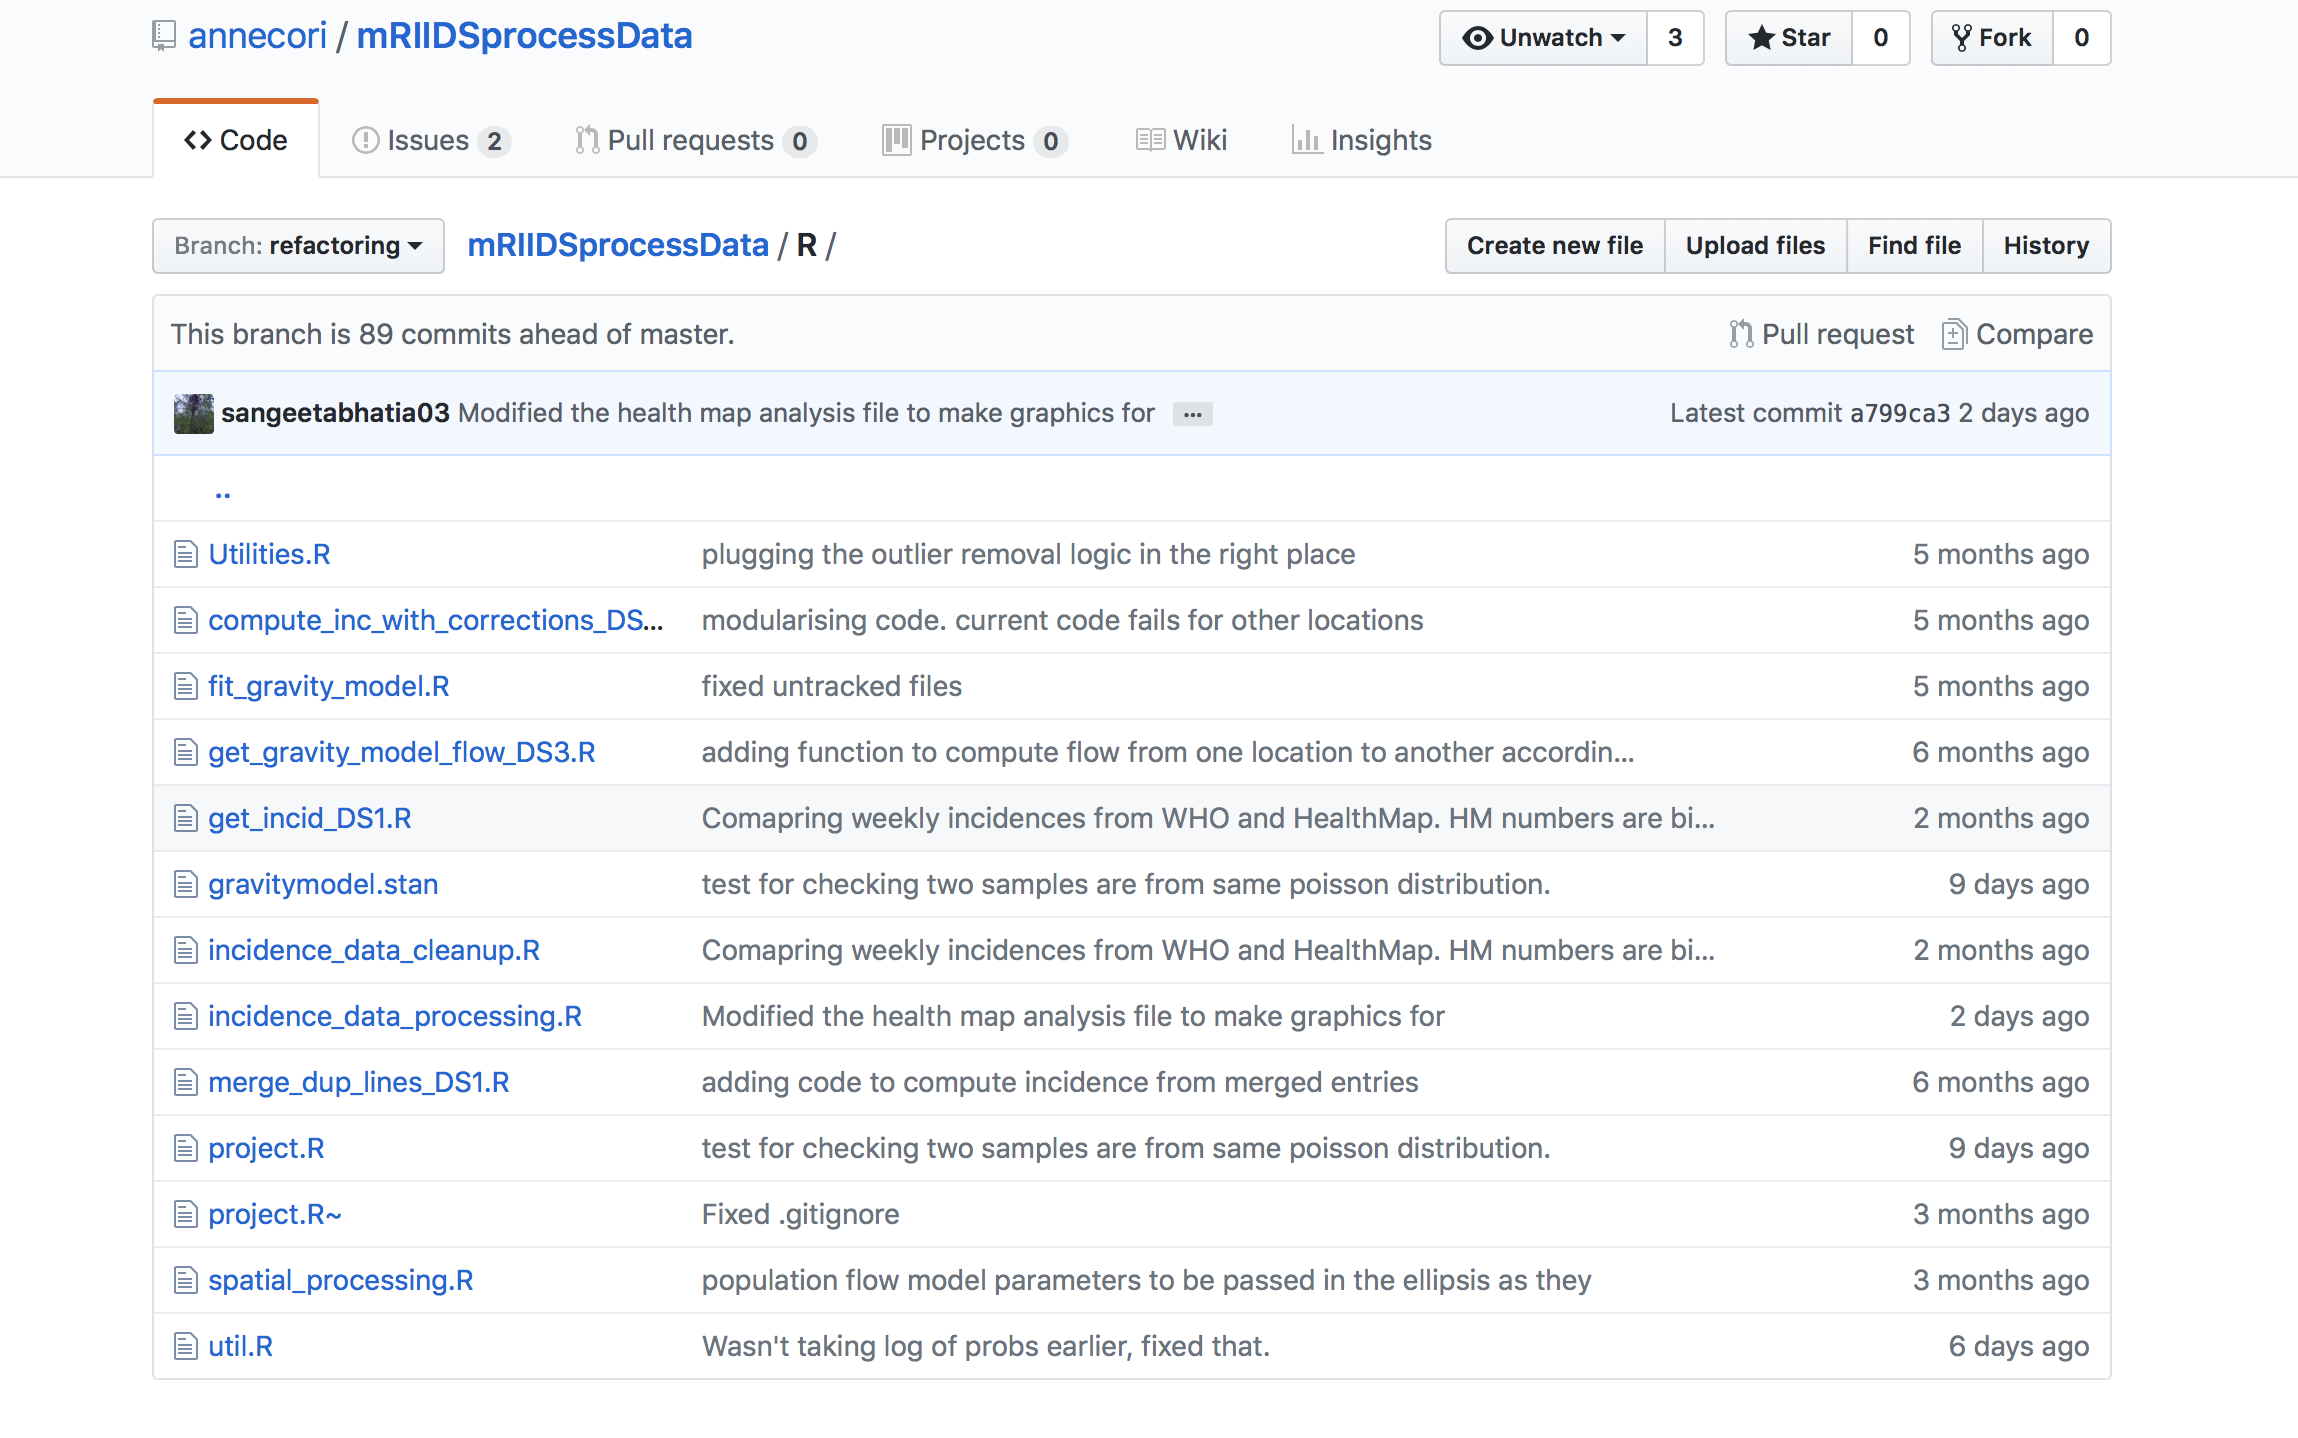
\includegraphics[width=8cm, height = 6cm]{ms6-figures/github-screenshot}
  \caption{The software being developed for the project is available
    on GitHub.}
  \label{fig:github}
\end{figure}


The package will include extensive documentation in the form of
user-friendly help files and vignettes. An example of a help file can
be seen in Figure~\ref{fig:helpfile}.


\begin{figure}
  \centering
  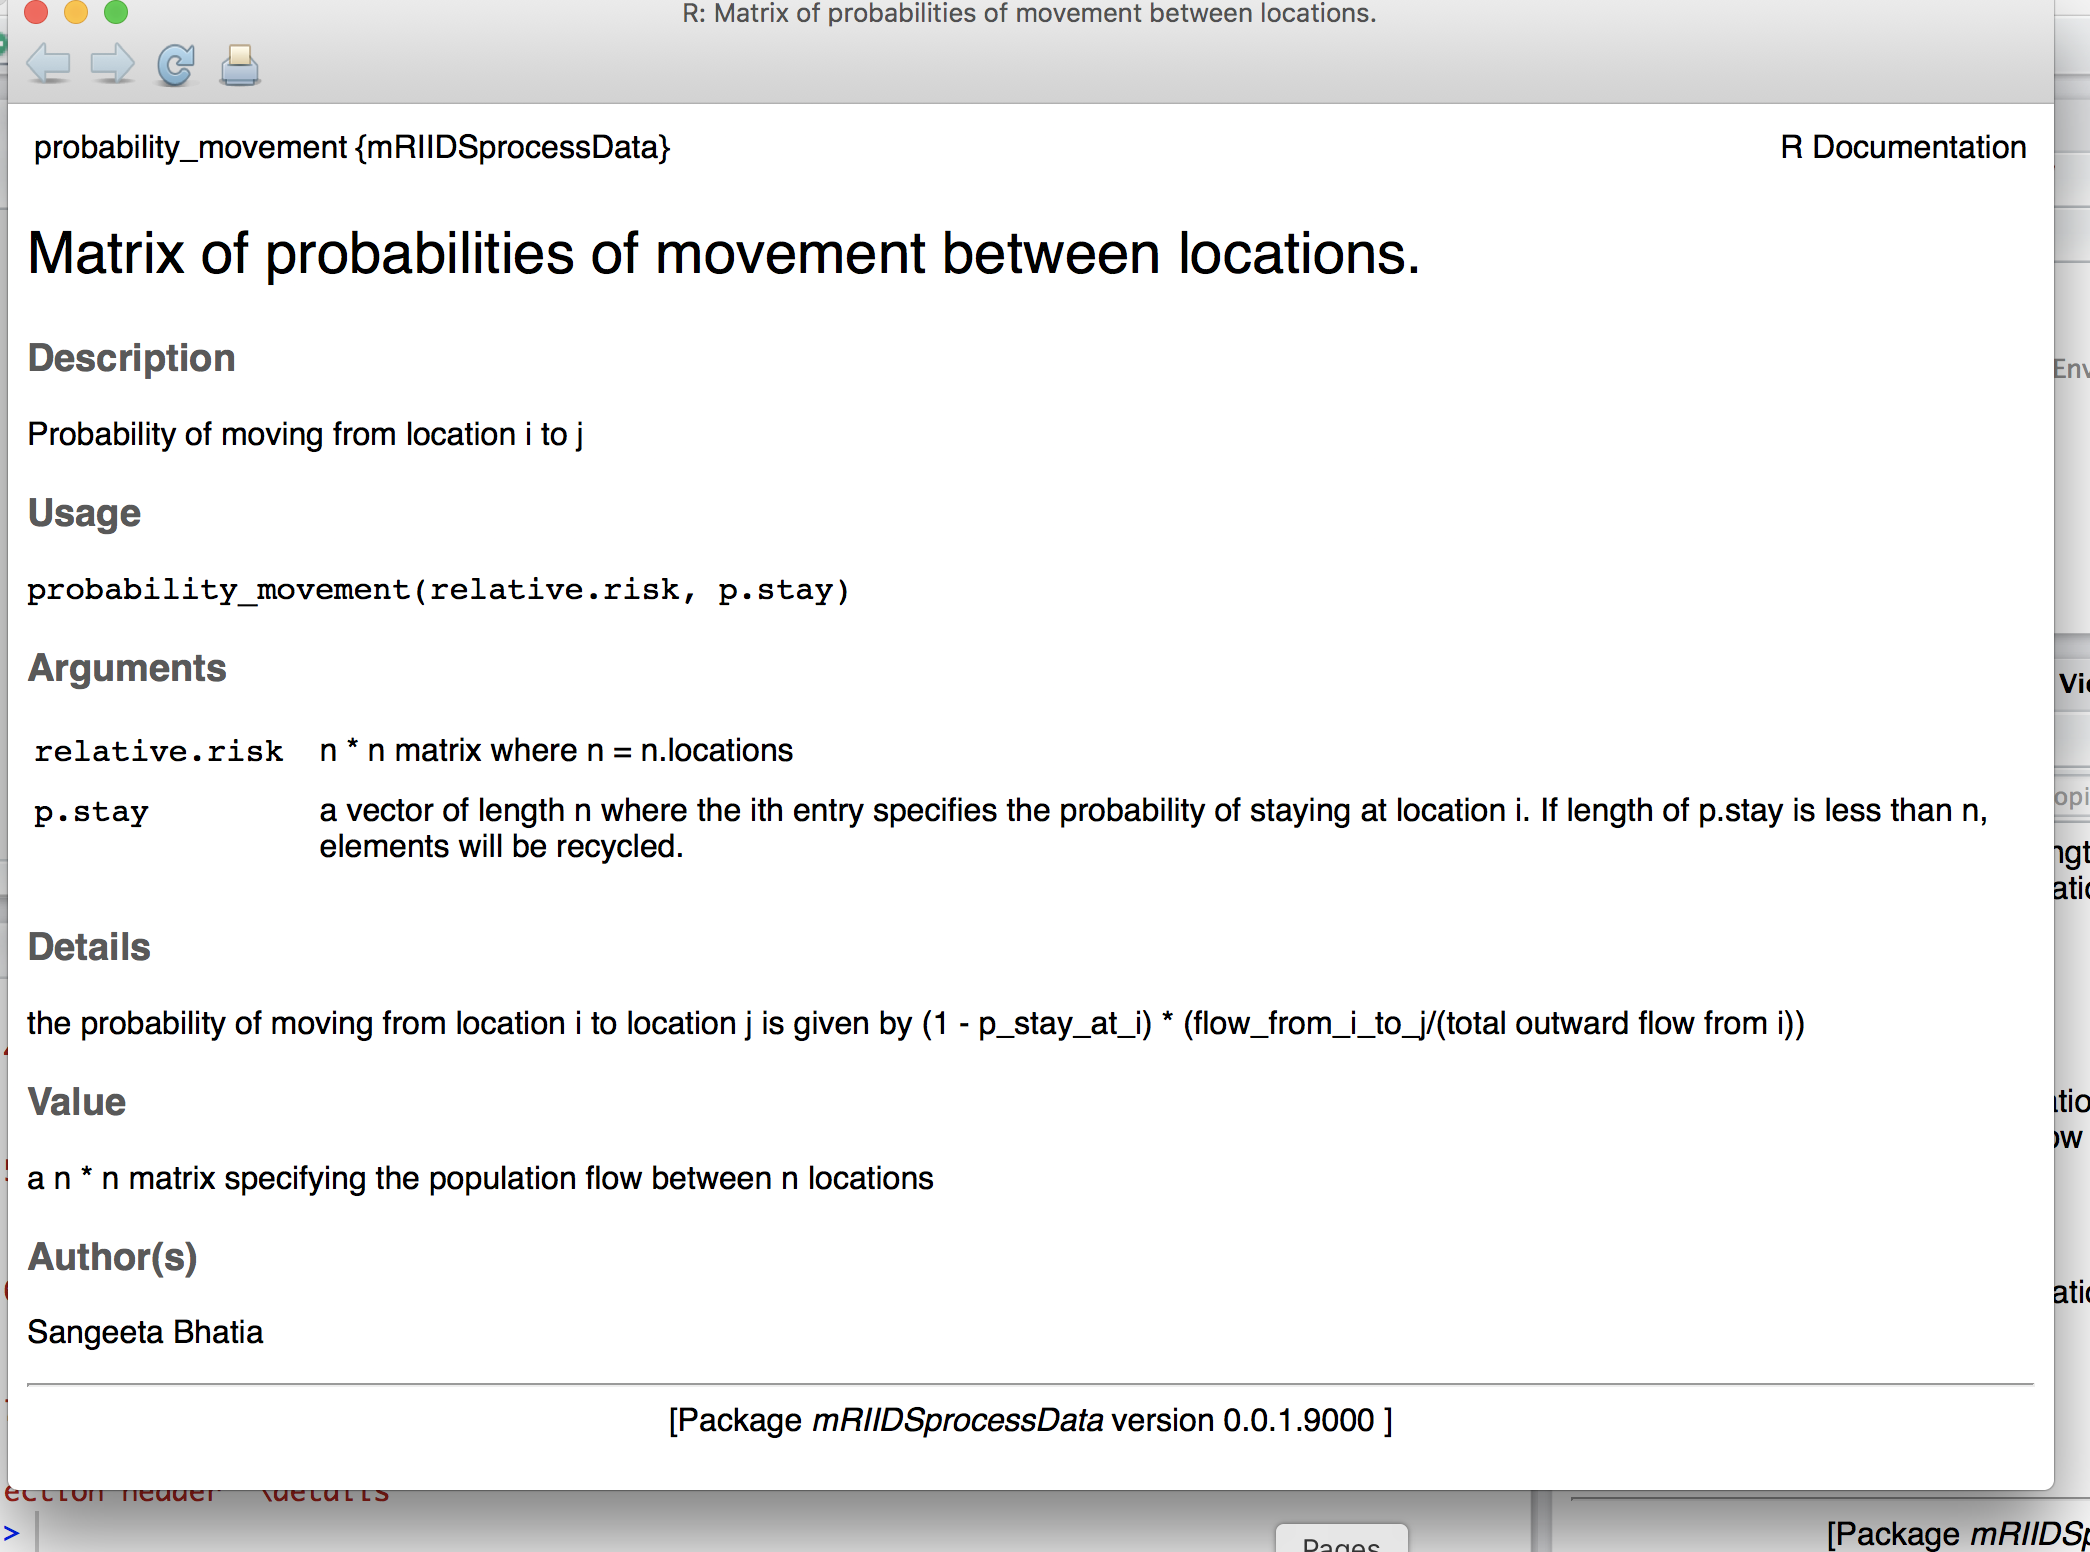
\includegraphics[width=8cm, height = 6cm]{ms6-figures/Helpfile-screenshot}
  \caption{An example of the documentation for the R package mRIIDS}
  \label{fig:helpfile}
\end{figure}

\FloatBarrier
\subsection{Collating data for each data stream}
\begin{center}
\begin{figure}
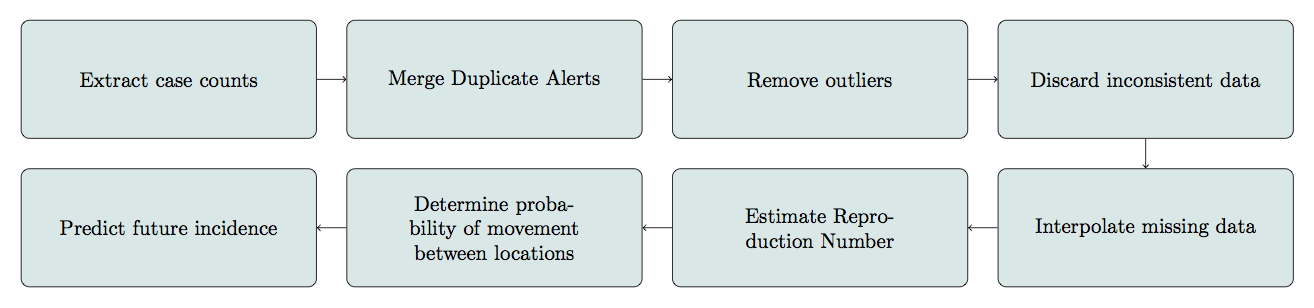
\includegraphics[]{ms6-figures/workflow}
\caption{Workflow for the processing of the various data streams.}
\label{fig:workflow}
\end{figure}
\end{center}

Figure~\ref{fig:workflow} summarizes the steps involved in collating
the different data streams and in going from raw data to predictions. In Milestone 6, a step was added to the data pre-processing workflow
to remove outliers from data. The removal of outliers was done using Chebyshev Inequality
with sample mean (see~\citep{saw1984chebyshev}). Figure~\ref{fig:wf_example} illustrates
the results of each step in the pre-processing steps in the workflow.

\begin{figure}
  \centering
  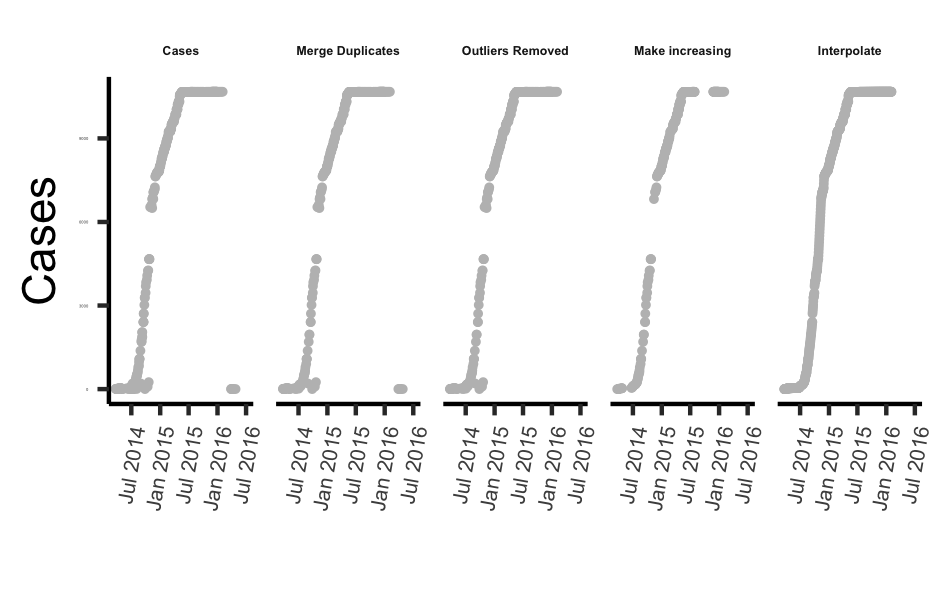
\includegraphics[]{ms6-figures/liberia-preprocessing2}
  \caption{Illustration of the pre-processing steps on HealthMap incidence
    data for Liberia.}
  \label{fig:wf_example}
\end{figure}
\FloatBarrier

\subsection{Model training and validation using data from
WHO}\label{model-training-and-validation-using-data-from-who}

In the current iteration, the model was trained and validated the data
on cases officially reported to the WHO during the 2013--2016 Ebola
outbreak in Guinea, Liberia and Sierra Leone. This dataset was cleaned
and published in \citep{garske20160308} and it is this cleaned version
of the data that were used in this work. This dataset consists of
incidence reports at ADM2 level. Thus in using it, we were able to validate the model at a finer spatial resolution than available
with HealthMap/ProMED data. We refer to this dataset as WHO data
throughout the rest of this document.

For data stream 2 i.e., parameters informing the transmissibility of
Ebola, we assumed a Gamma distributed serial interval with mean 14.2
days and standard deviation 9.6 days \citep{team2015west}.
As in Milestone 4, a Gamma prior with mean 3.3 and variance 1.5 was
used for the reproduction number. This was informed by a review of estimates of the reproduction number for Ebola Zaire in outbreaks preceding the West African Ebola outbreak \citep{van2015review}, which reported estimates ranging from 1.4 to 4.7. The mean prior 3.3 was chosen as the midpoint of this interval, and the variance 1.5, was chosen so the 95\% prior probability interval contains the extremes of this interval.



\subsection{Incidence trends from different data sources}
We aggregated the WHO data to national level to compare the incidence
trends derived from the three different data sources (WHO, HealthMap
and ProMed). As can be seen in Figure~\ref{fig:incid_comp}, the incidence time series
of the three data sources were well correlated.

\begin{figure}
    \centering
        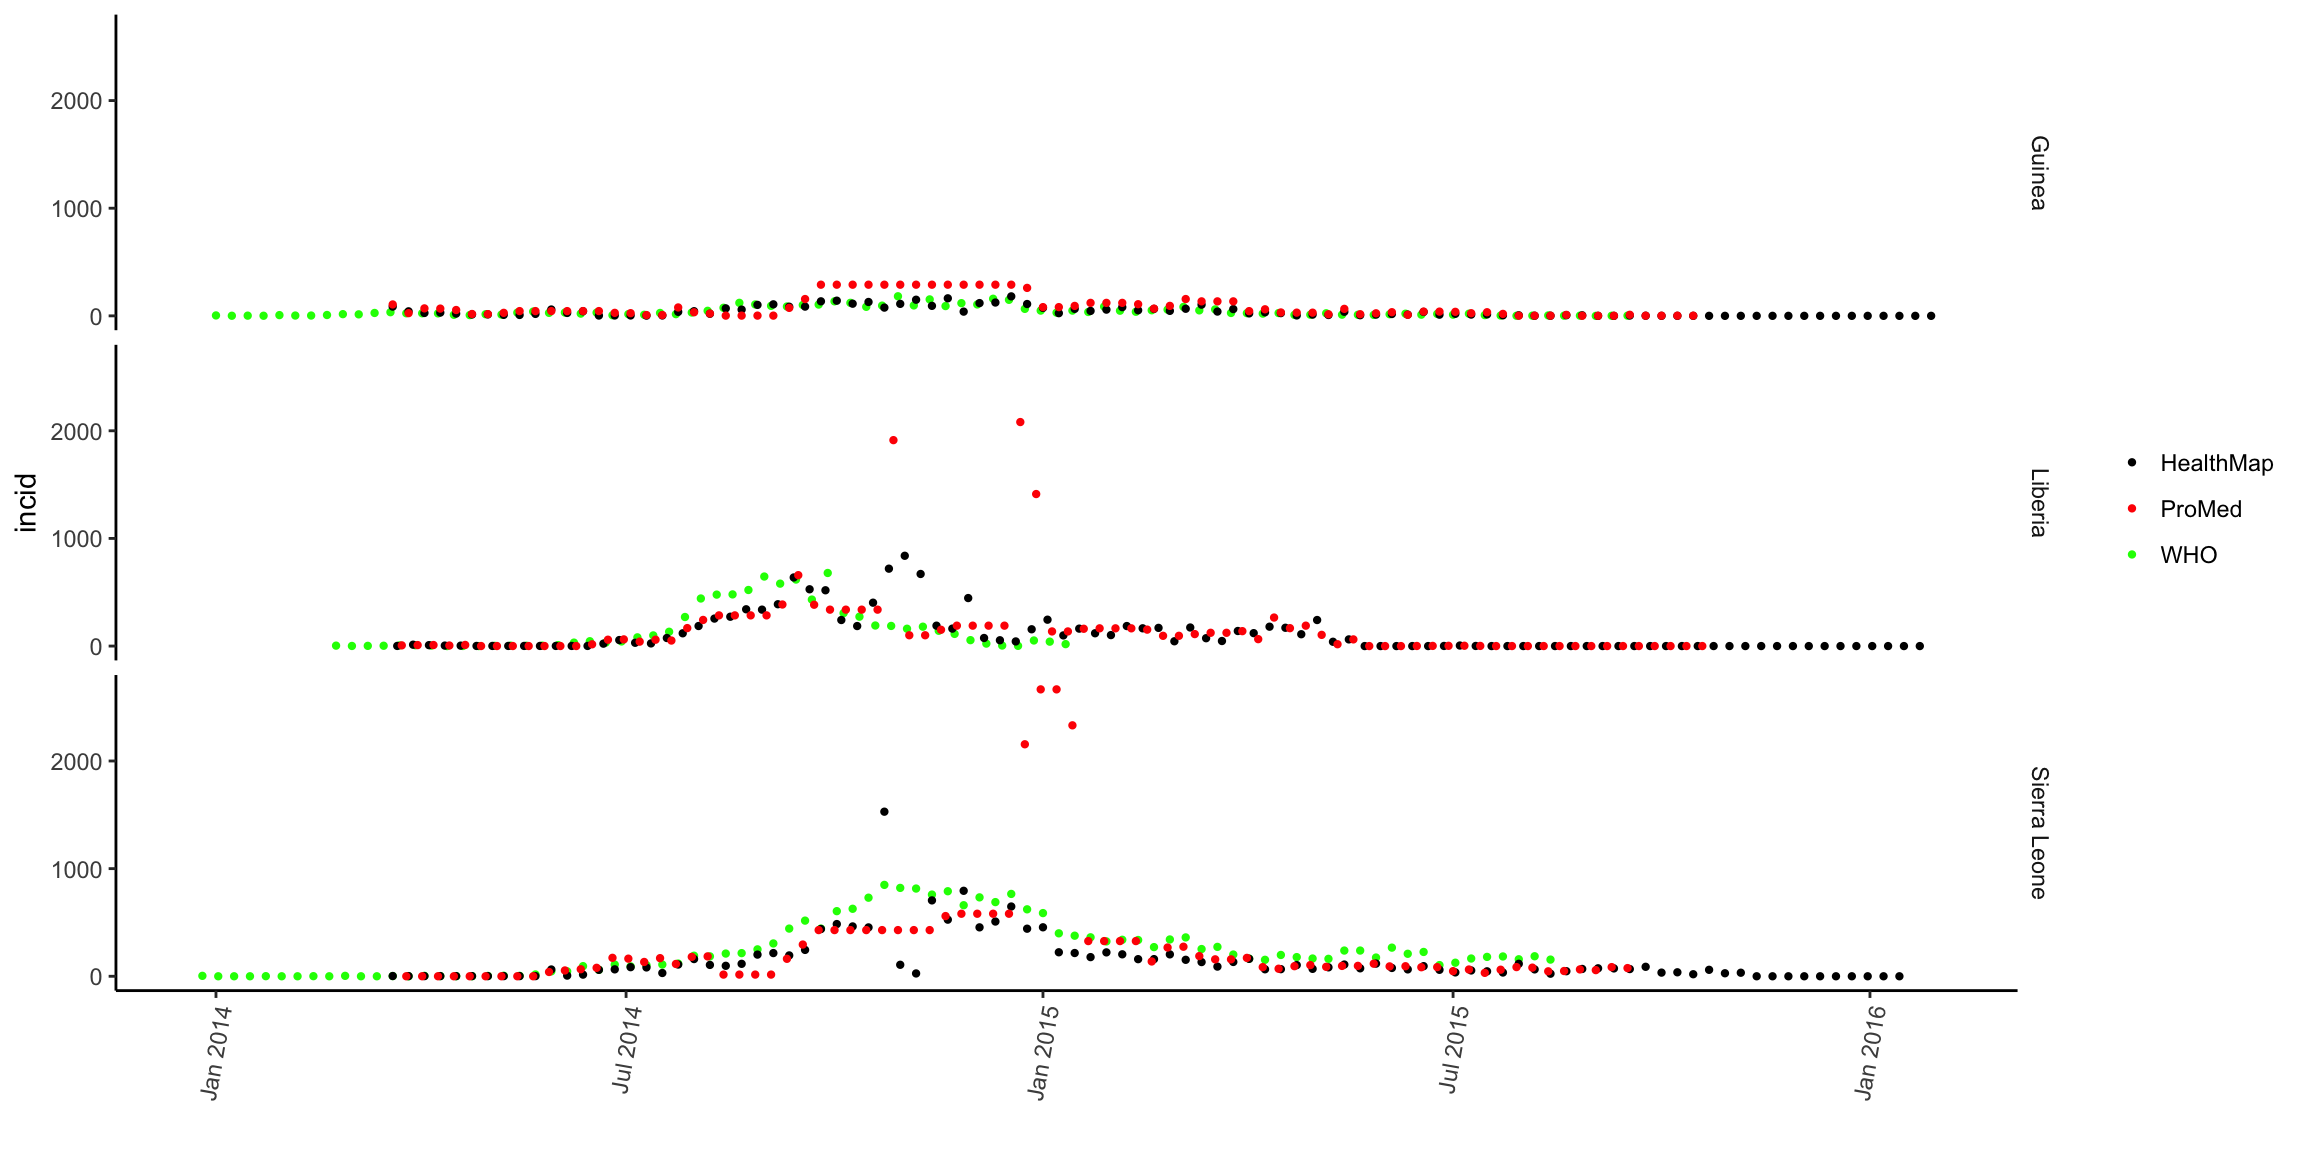
\includegraphics[]{ms6-figures/who_hm_pm_weekly_incid-1}
        \caption{Comparison of weekly incidence data from WHO, HealthMap and ProMed.}
        \label{fig:incid_comp}
  \end{figure}

During an emergency, such as the West Africa epidemics, spatially refined data (such as the WHO data)
are typically not available in real time due to reporting delay \citep{cori2017key}. A key advantage 
of relying on ProMED/HealthMap data in our project is the real time nature of the data. However this come at the cost
of nationally aggregated data.

The results of the analysis above point toward a potential solution to obtain `pseudo real-time' district
 level incidence data. One could relay on real-time national data (e.g. ProMED/HealthMap) and disaggregate 
the time-series to obtain district level incidence using spatial information from a `retrospective'
time-series at finer scale (i.e. WHO data).
\FloatBarrier
\subsection{Inference of parameters}

The parameters of the full model detailed in Section~\ref{sec:model} are
$\alpha$, $\beta$, $\gamma$, $p_{stay}$ and $R_{i, t}$. A simple
estimation of $R_{i, t}$ can be obtained using incidence data and knowledge of the serial interval.
Such statistical procedure has been implemented in the
R package EpiEstim. Figure~\ref{fig:r_comp} shows the
reproduction number estimated assuming constant transmissibility during period of 28 days. 
Sliding  28 days windows allow us to obtain daily estimate of the reproduction number (see \citep{cori2013new} for details).

We estimated temporal pattern of the reproduction number for the 3 most affected country in West Africa
using either data sources (Promed, HealthMap, and WHO).
The high degree of correlation in the estimates of transmissibility from the three
different data sources shows that the estimation procedure is robust
to slight variations in reported incidence.

\begin{figure}
  \centering
  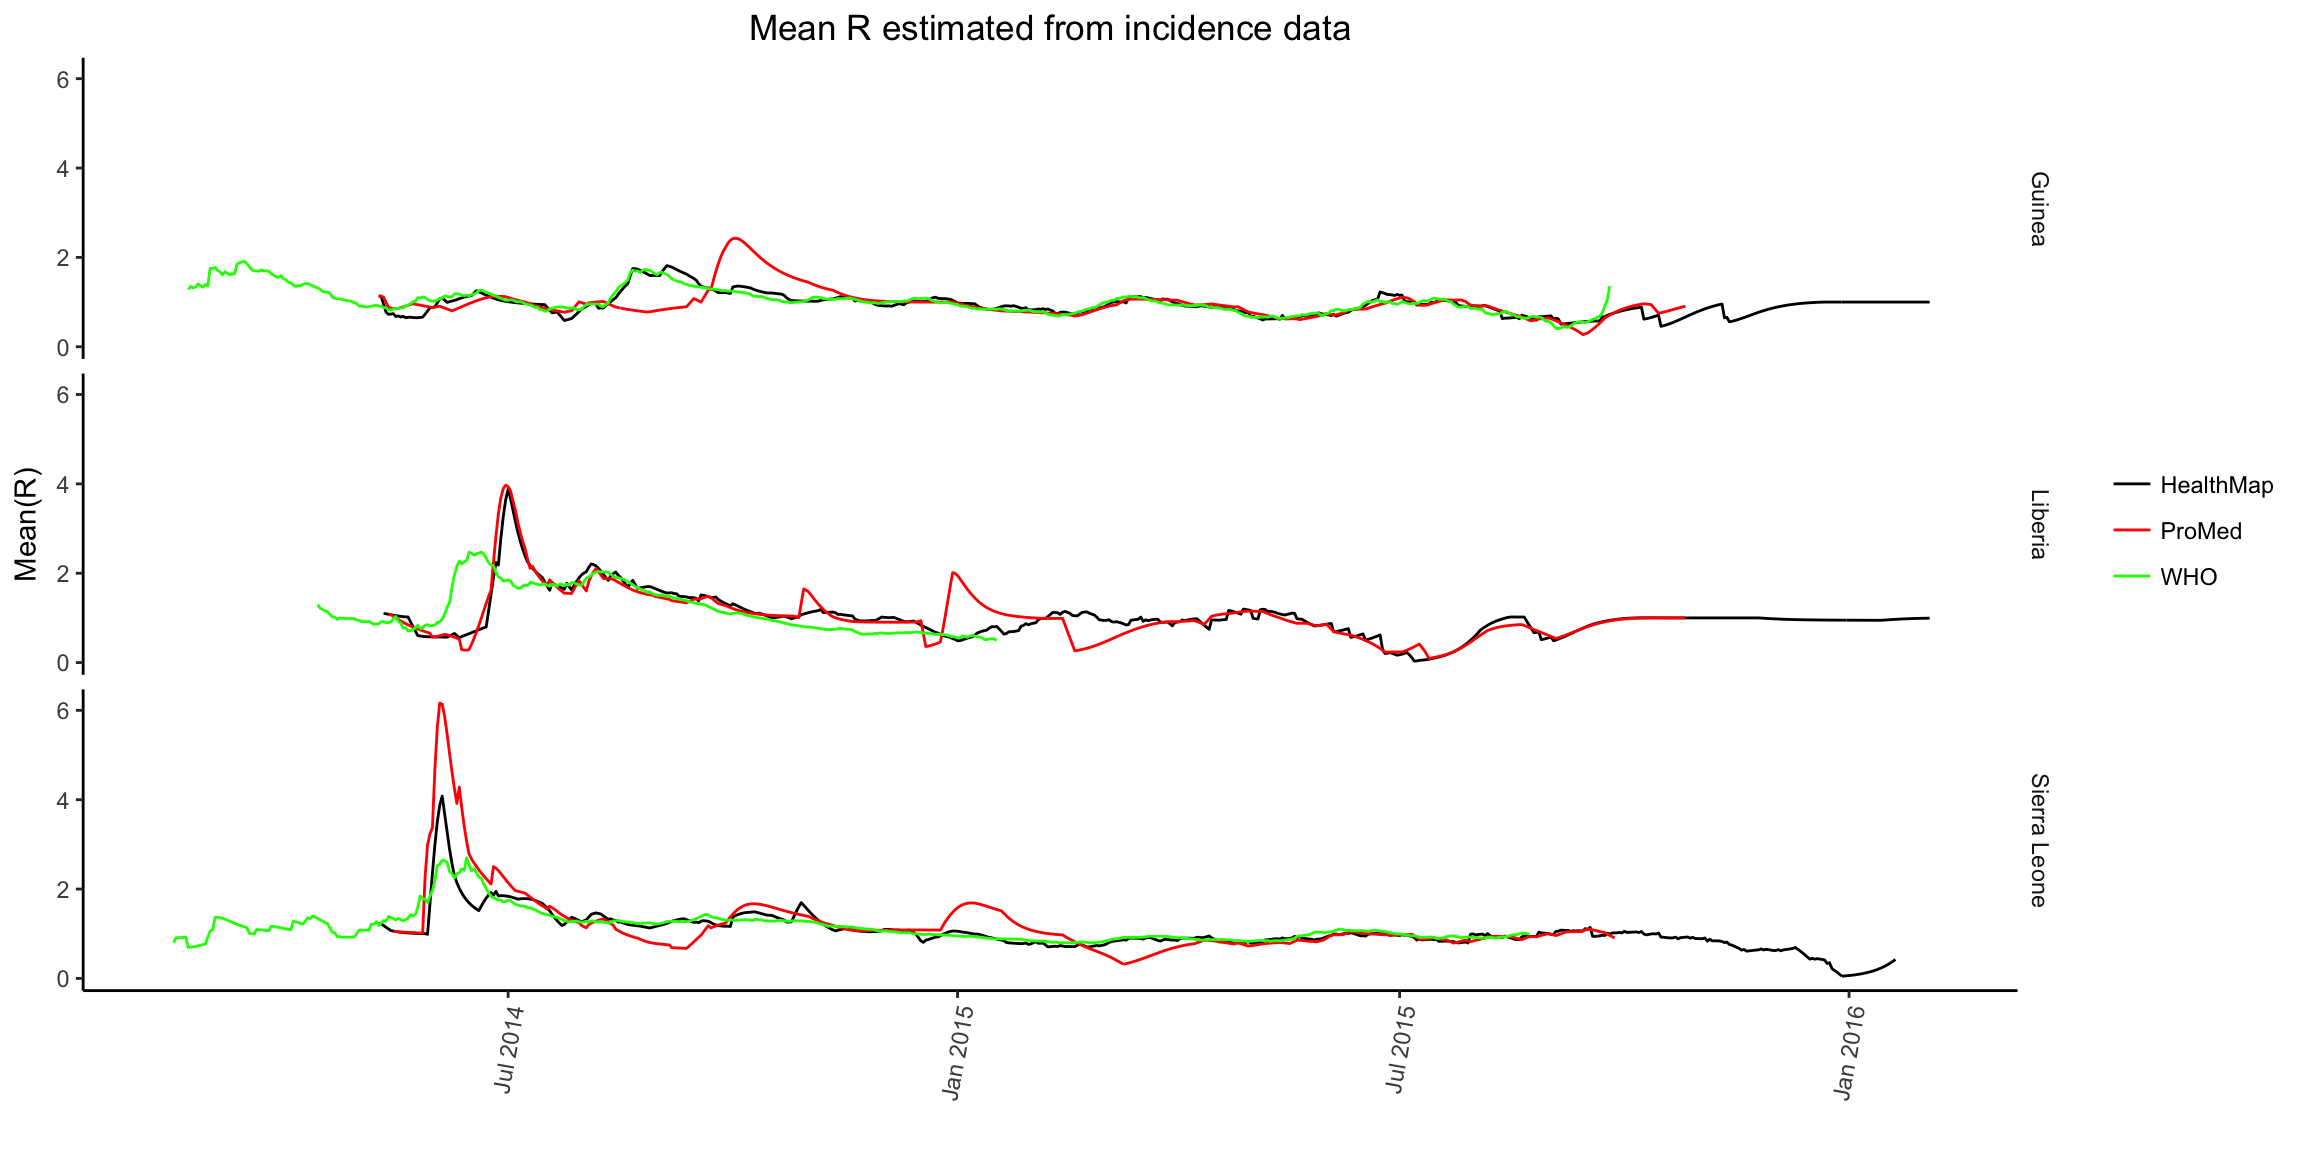
\includegraphics[width=\textwidth]{ms6-figures/who_vs_hm_vs_pm-1}
  \caption{Comparison of the reproduction numbers estimated from
        the different sources of the incidence data.}
  \label{fig:r_comp}
\end{figure}

\FloatBarrier
Then, the spatial spread must be assessed.
In the interest of simplicity, we assume both
$\alpha$ and $\beta$ to be $1$. The other two parameters are
$p_{stay}$ and $\gamma$. We explored the influence of these two
parameters on the quality of fit of the predictions from the models at various points in the
epidemic. To assess the goodness-of-fit, we used the normalised root mean squared
error (rms), which is the sum of squares of the differences between
observed and predicted values. That is, 
\[ rms := \sum_{i = 1}^n{\left(o_i - p_i\right)^2},\]
where $o_i$ is $i$th observation, $p_i$ is the corresponding value
predicted by the model and $n$ is the total number of observations.

\begin{figure}
  \centering
  \begin{subfigure}[b]{0.4\textwidth}
    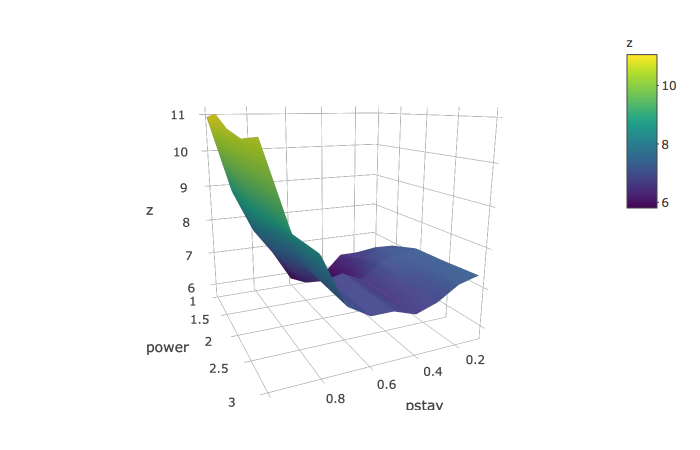
\includegraphics[]{ms6-figures/rms-100-2}
    \caption{Root mean square errors for prediction for 5 weeks at 100 days from the start of the epidemic.}
    \label{fig:rms-100}
\end{subfigure}
~
  \begin{subfigure}[b]{0.4\textwidth}
    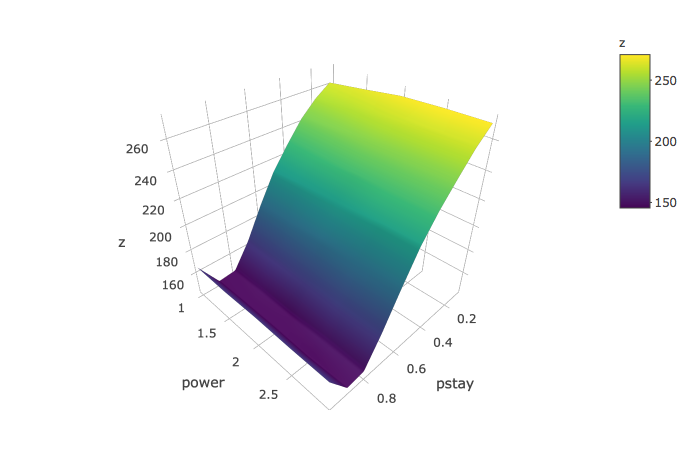
\includegraphics[]{ms6-figures/rms-300-2}
    \caption{Root mean square errors for prediction for 5 weeks at 300 days from the start of the epidemic.}    
    \label{fig:rms-300}
\end{subfigure}
  \caption[RMS as a function of model parameters]{Normalised root mean
    squared error as a function of the model parameters. The fit is
    assessed for prediction of 5 weeks at 100 and 300 days from the start of
    the epidemic. The fit is better for smaller values of the root
    mean square error. In the early phase of the epidemic, a better
    fit is obtained at a smaller value of $p_{stay}$ while at the 300
    days mark, a much higher value of $p_{stay}$ is needed to obtain a
  good fit.}
  \label{fig:rms}
\end{figure}
\FloatBarrier
\subsection{Predicting Future Cases}\label{predicting-future-cases}

As mentioned earlier, the WHO data consisted of incidence data at the district level. To
validate the model, we carried out analysis at both the district level
using WHO data and at country level using data from HealthMap.

\subsubsection{Prediction at country level}

Predictions over a 7 week period were carried out using the incidence
data provided by HealthMap. The results for Sierra Leone, Liberia and
Guinea are presented here. The data pre-processing steps detailed in
an earlier section were applied. The incidence obtained after these
steps are shown in Figure~\ref{fig:hm-incid}.

\begin{figure}
  \centering
  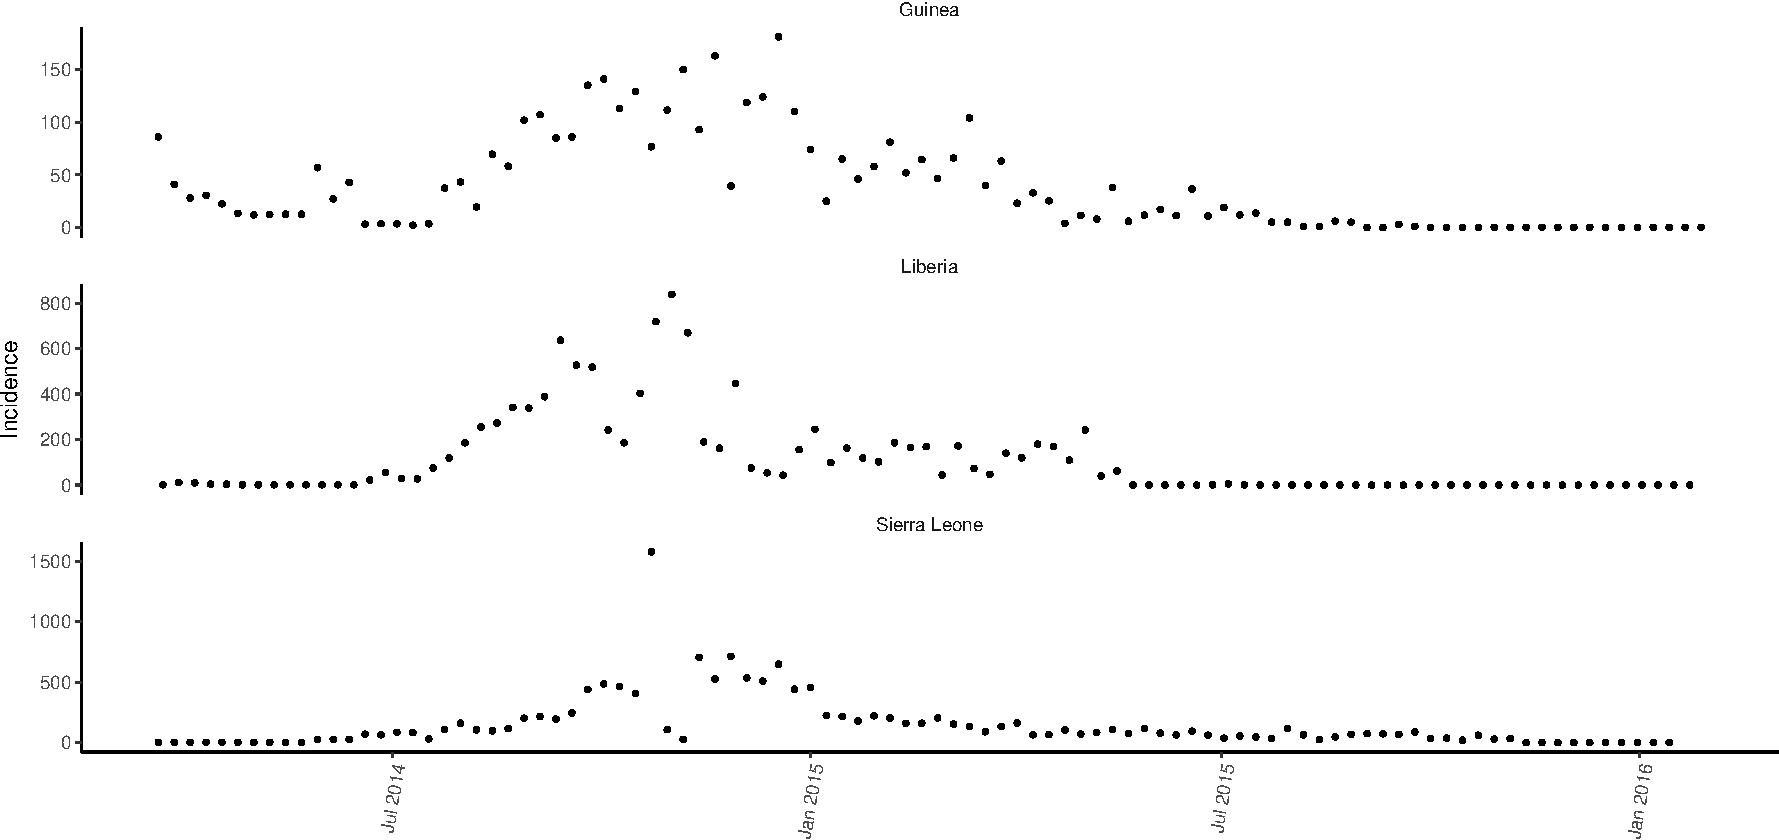
\includegraphics[]{ms6-figures/hm_weekly_incid-1}
  \caption{Weekly incidence data from HealthMap after the pre-processing
    steps.}
  \label{fig:hm-incid}
\end{figure}

The projection was done at two
different time steps - at 150 days and 400 days from the start of the
epidemic (August 2014 and April 2015
respectively) in order to capture an increasing as well as a
decreasing phase in the outbreak. Figure~\ref{fig:hm-prediction-200} shows the
predictions for October 2014. Figure~\ref{fig:hm-prediction-400} is
the corresponding figure for projections in April 2015.

\begin{figure}
  \centering
  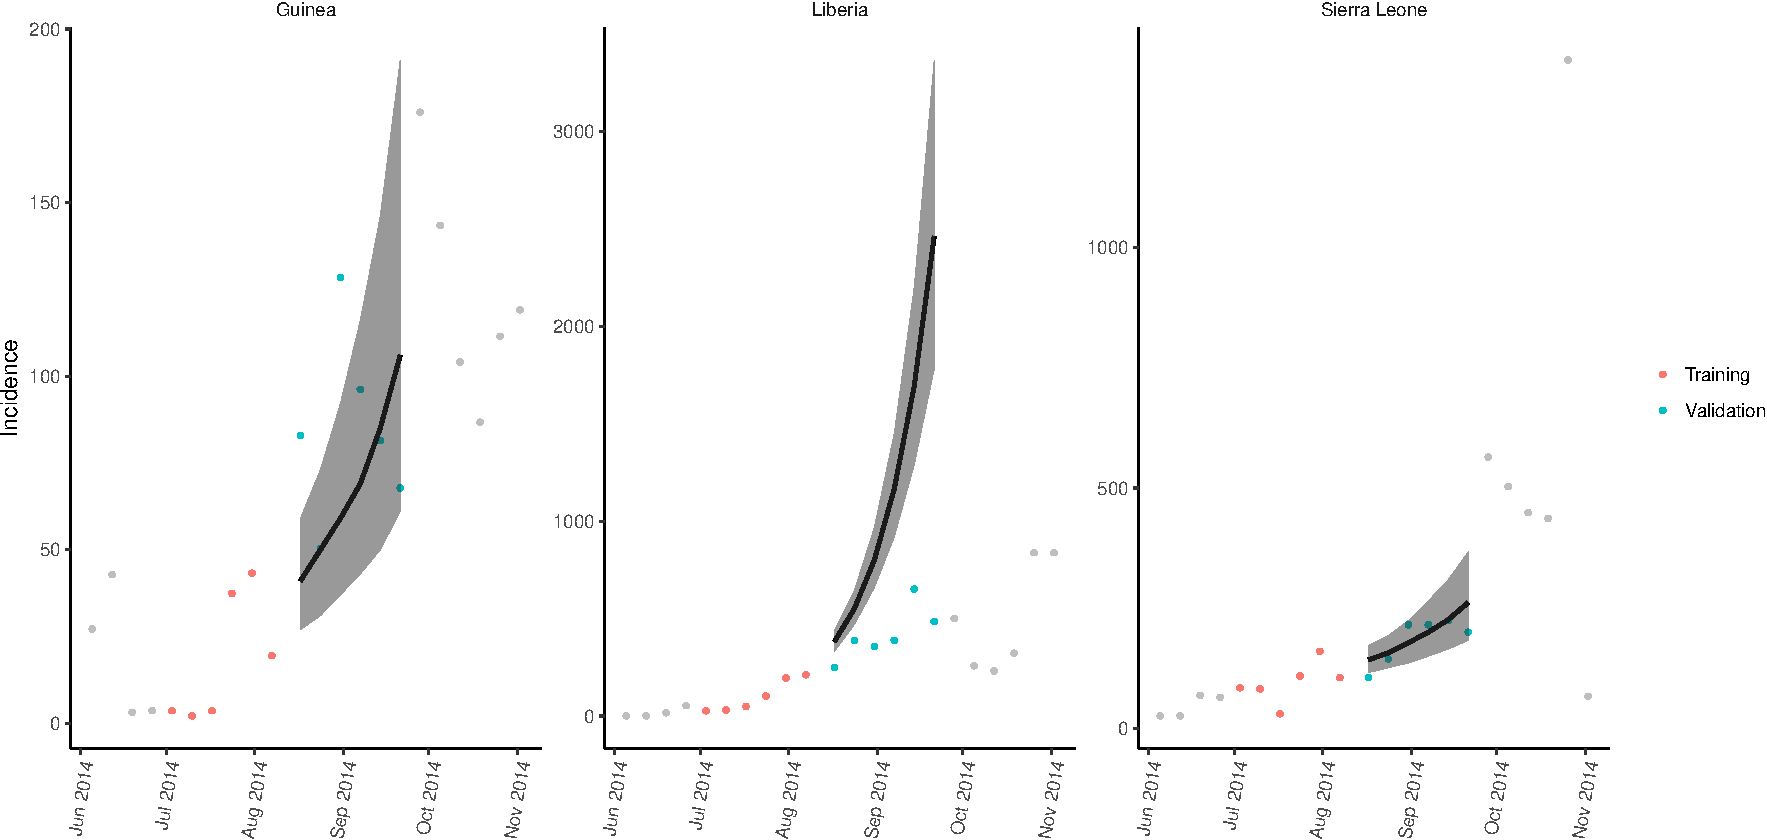
\includegraphics[]{ms6-figures/hm_summary_projections_0.99_1_150}
  \caption{Predictions using HealthMap data in August 2014. The
    orange dots represent the data used to estimate the instantaneous
    reproduction number. The blue dates represent the observed
    incidence in the period over which prediction is being carried
    out. The solid black line traces the median projected incidence
    and the shaded area constitutes the 95\% credible interval around
    the median incidence.}
  \label{fig:hm-prediction-200}
\end{figure}


\begin{figure}
  \centering
  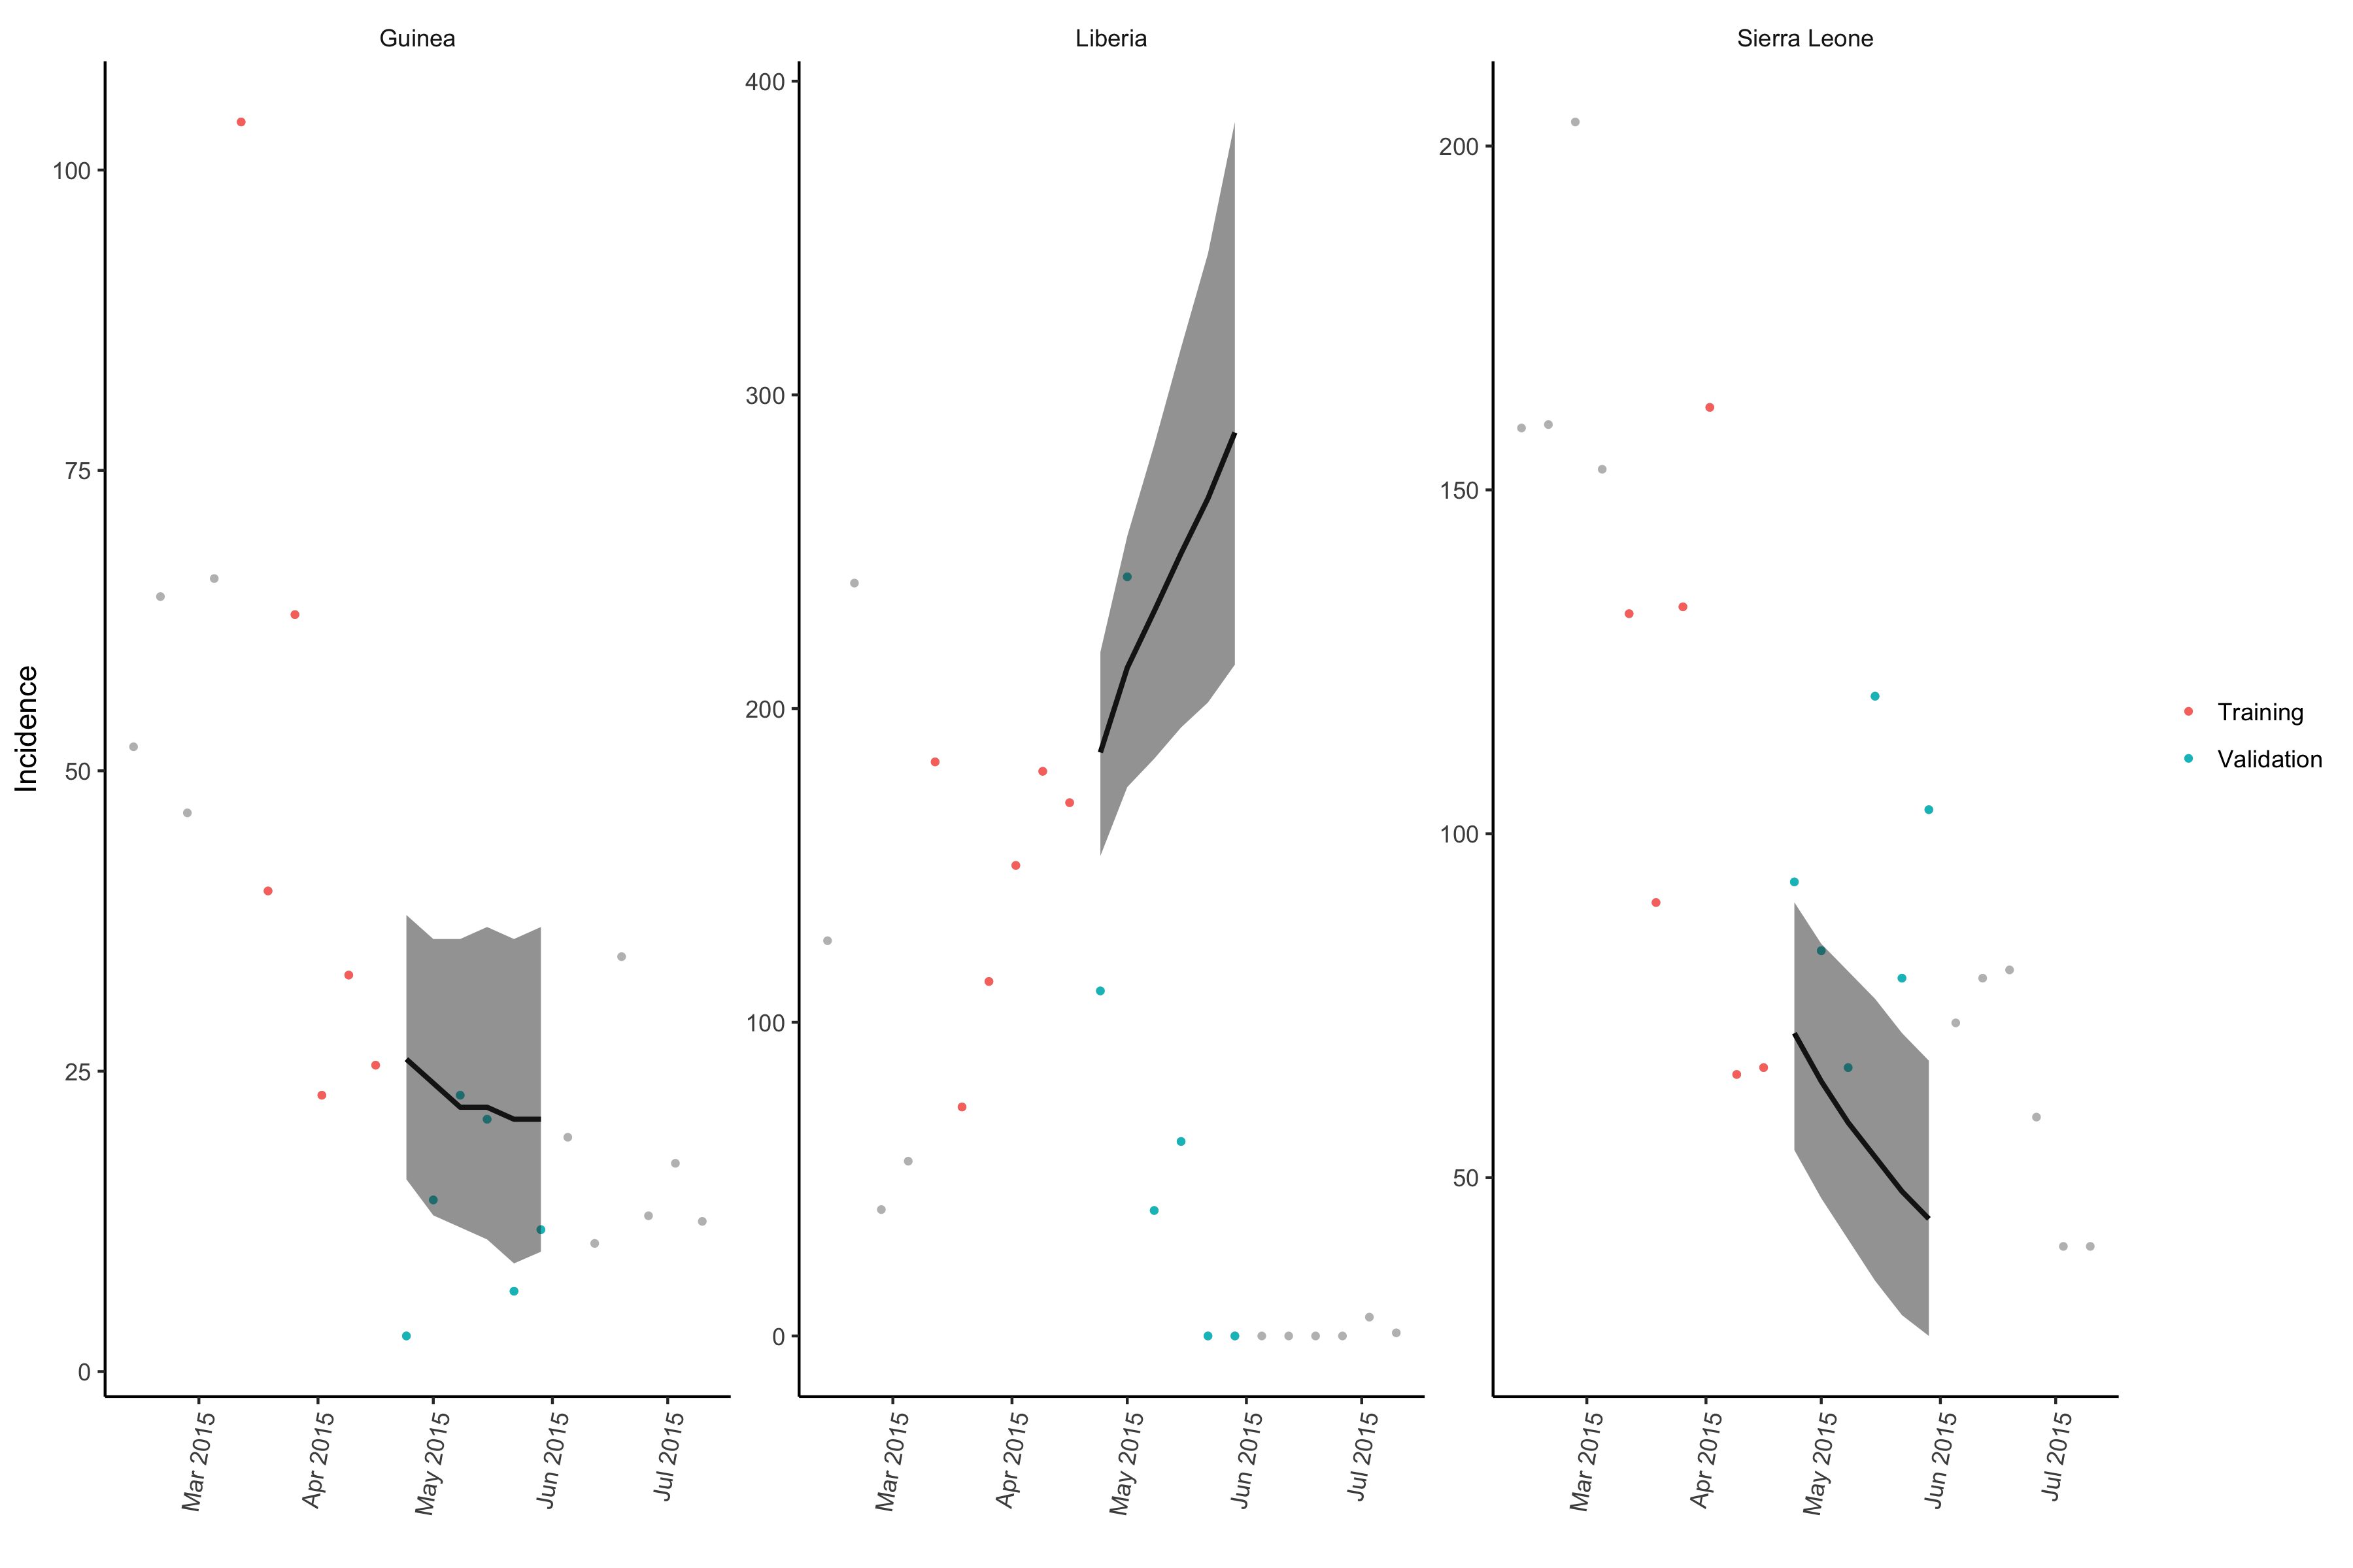
\includegraphics[]{ms6-figures/hm_summary_projections_0.99_2_400}
  \caption{Predictions using HealthMap data in October 2014. The
    orange dots represent the data used to estimate the instantaneous
    reproduction number. The blue dates represent the observed
    incidence in the period over which prediction is being carried
    out. The solid black line traces the median projected incidence
    and the shaded area constitutes the 95\% credible interval around
    the median incidence.}
  \label{fig:hm-prediction-400}
\end{figure}
\FloatBarrier
\subsubsection{Prediction at district level}

Predictions over a 7 week period were carried out at 2 different time points - at 300 and
500 days from the start of the epidemic (October 2014 and May 2015
respectively). It is assumed that the 
transmissibility did not change for the previous 7 weeks (as in
\citep{team2015west}). This analysis was carried at the sub-national
levels for Sierra Leone, Liberia and
Guinea as well as across the 55 districts in the three countries.
Figure~\ref{fig:sl-predictions} illustrates the results for
Sierra Leone.  Figure~\ref{fig:sl-map} compared the observed and
predicted spatial spread of the epidemic over a 7 week period
beginning in May 2015. It can be seen that the model performs well at
capturing the spatial dimension of the epidemic.

\begin{figure}
  \centering
  \begin{subfigure}{0.8\textwidth}
    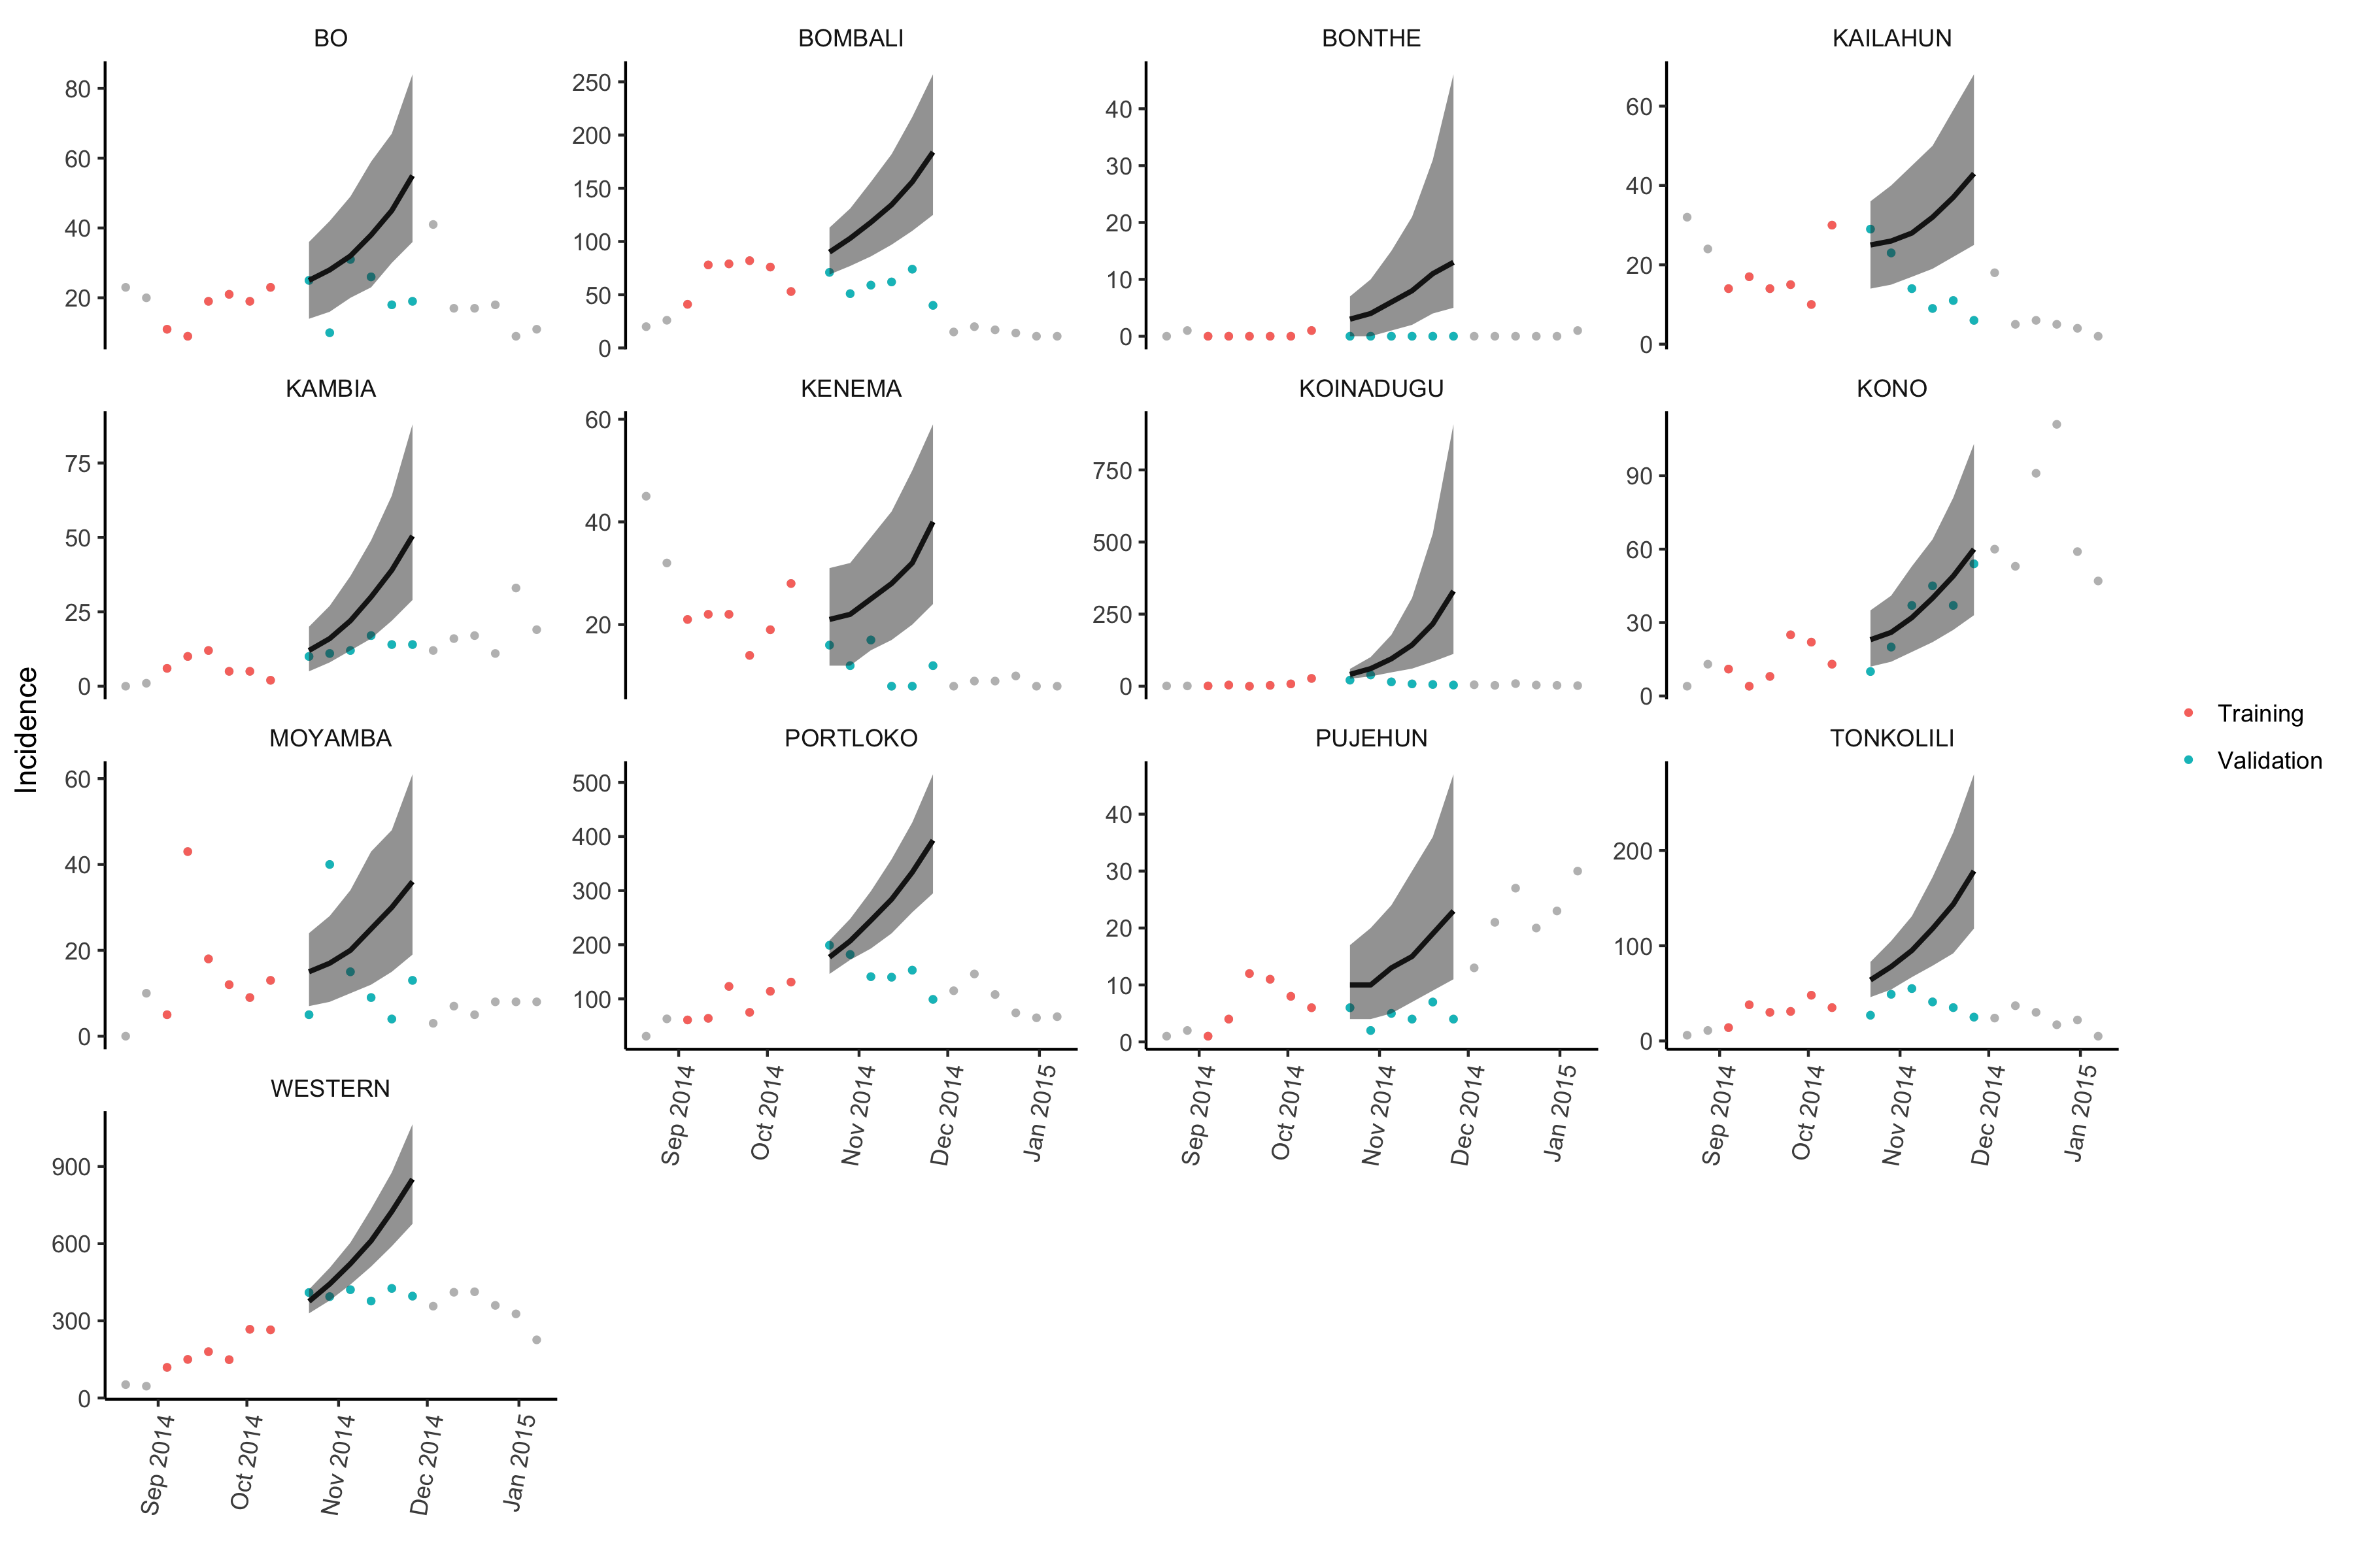
\includegraphics{ms6-figures/sl_summary_projections_0.9_1_300}
  \end{subfigure}
  ~
  \begin{subfigure}{0.8\textwidth}
    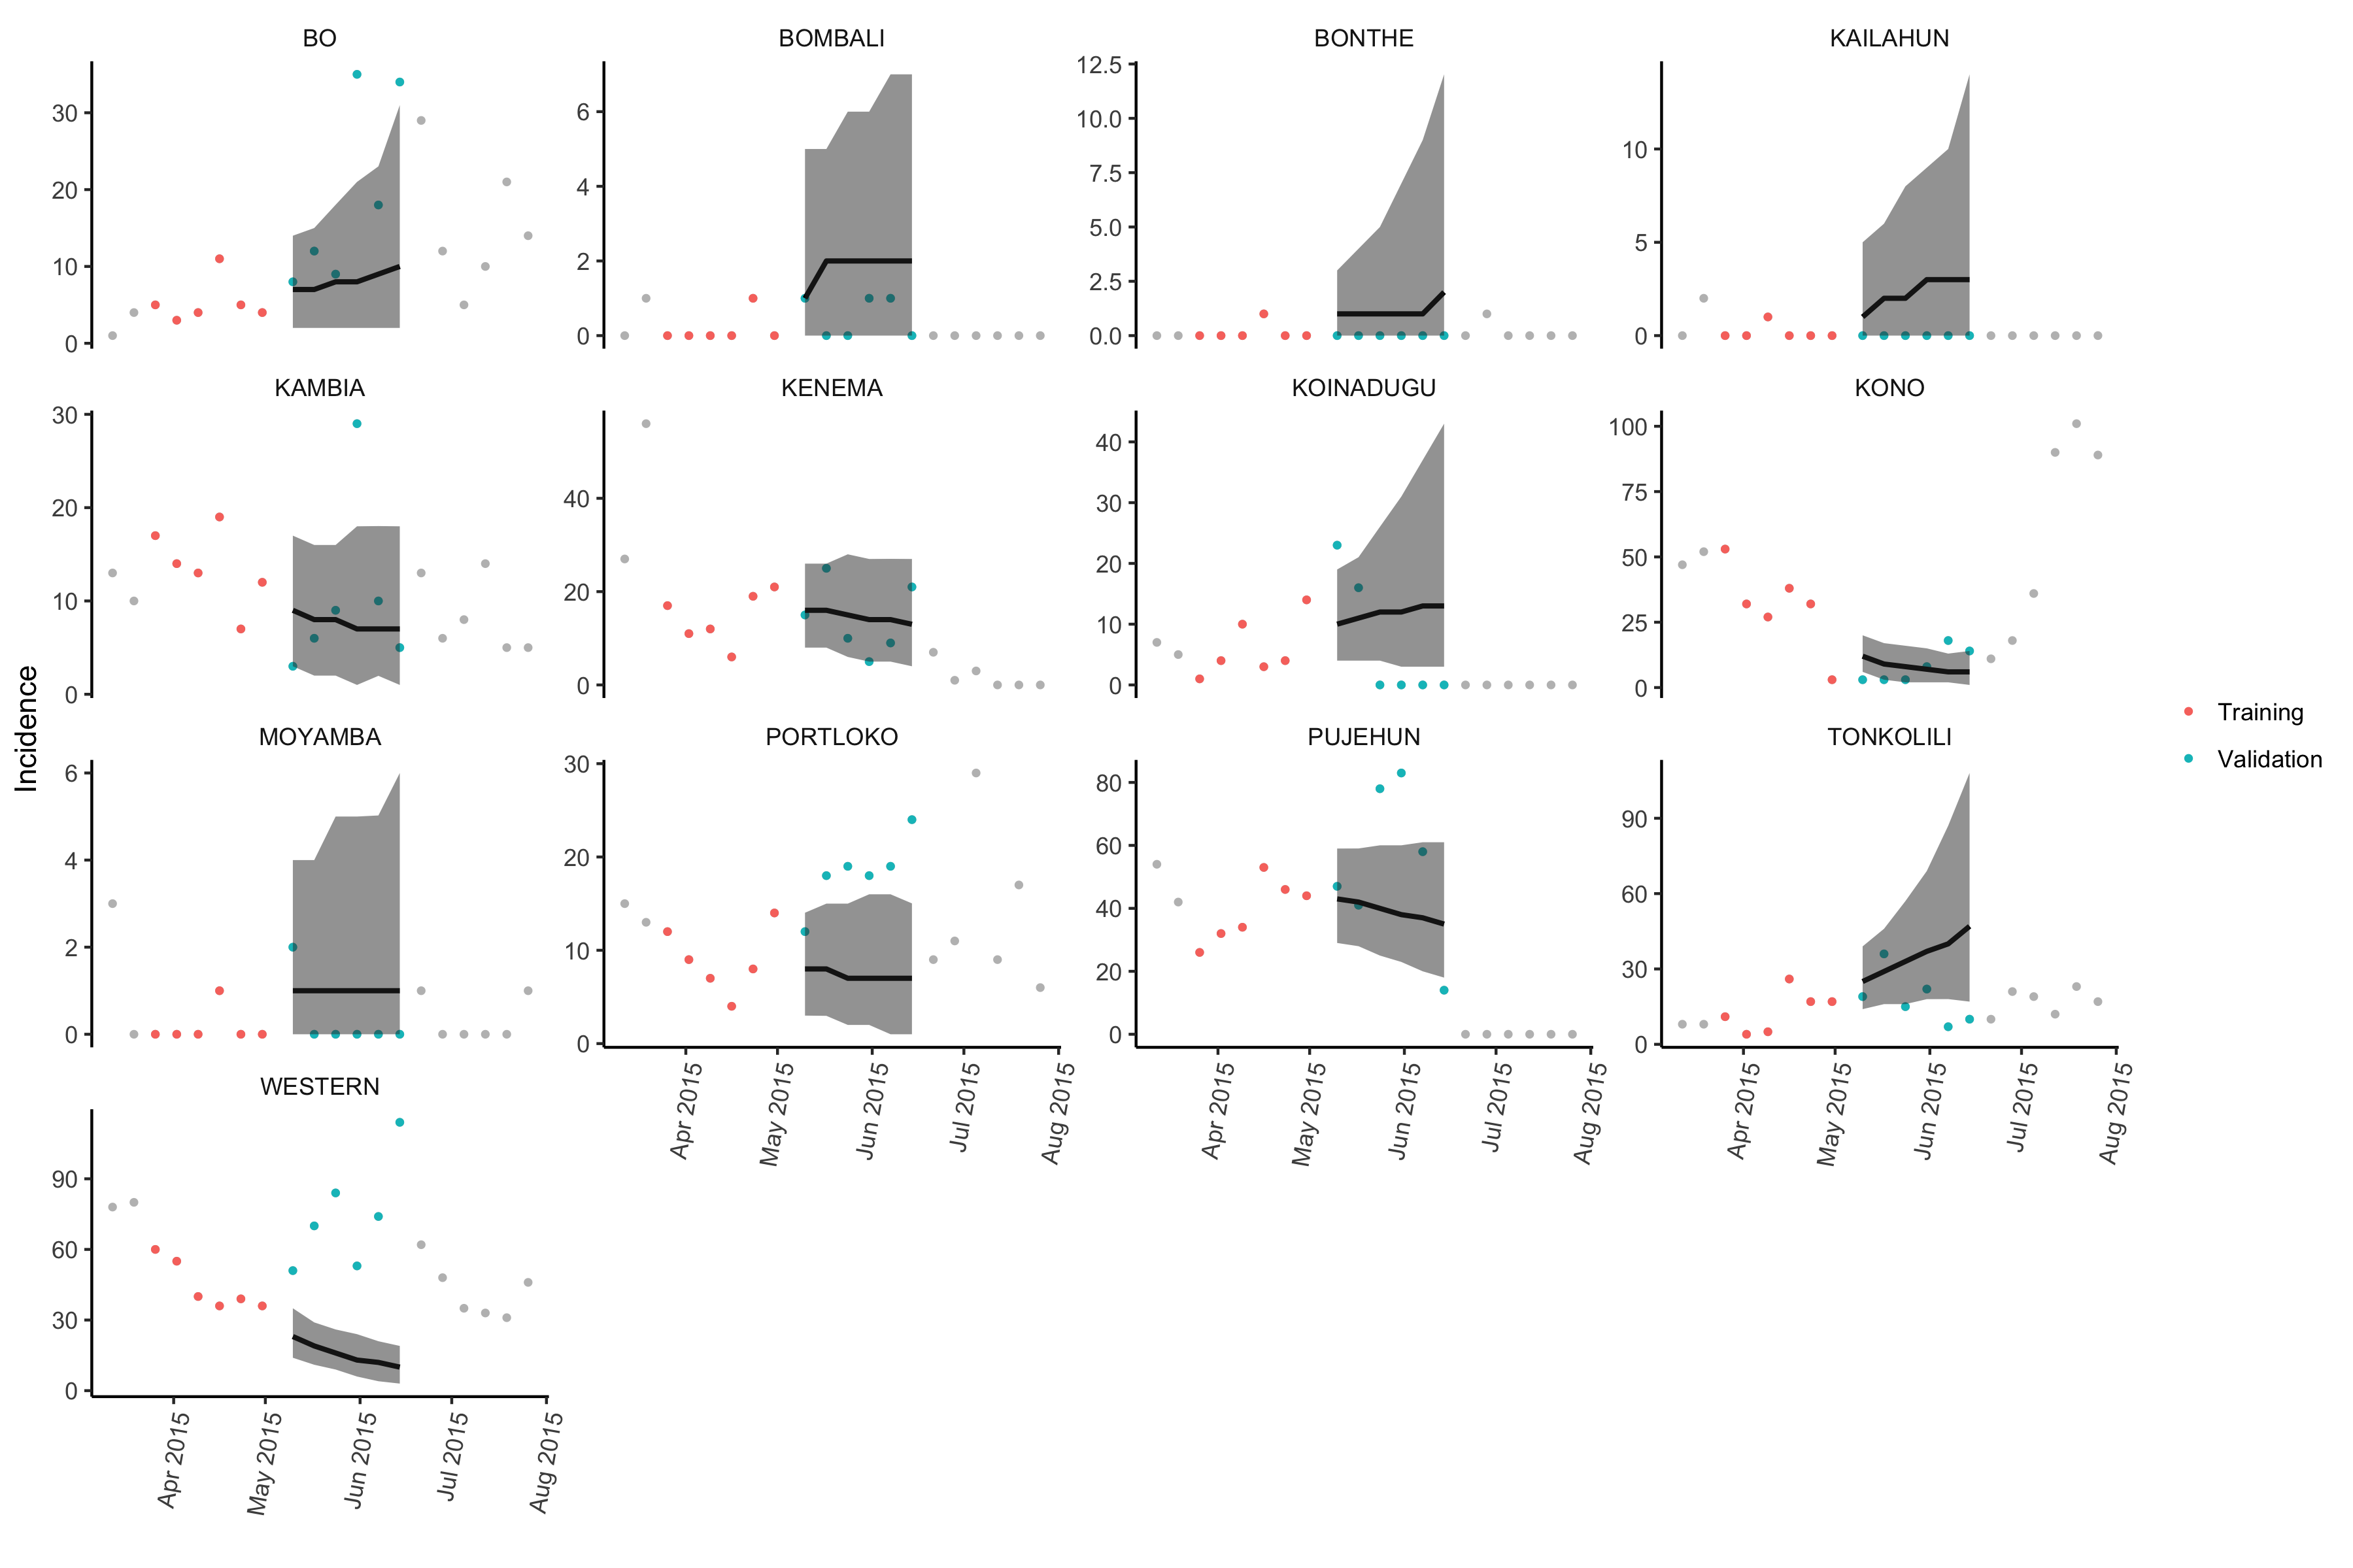
\includegraphics{ms6-figures/sl_summary_projections_0.9_1_500}
  \end{subfigure}  
  
  \caption[Sierra Leone Projections]{Spread of Ebola in the districts
    of Sierra Leone. Orange dots represent the data used to estimate
    the instantaneous reproduction number. Blue dots are the observed incidences in
    the period over which prediction is being carried out. Solid line
    represents the median predicted weekly incidence and the shaded
    area is the 95\% credible interval. The top panel shows the
    predictions at 300 days from the start of the epidemic (October
    2014) and the
    bottom panel is the prediction at 500 days (May 2015).}
  \label{fig:sl-predictions}
\end{figure}


\begin{figure}
  \centering
  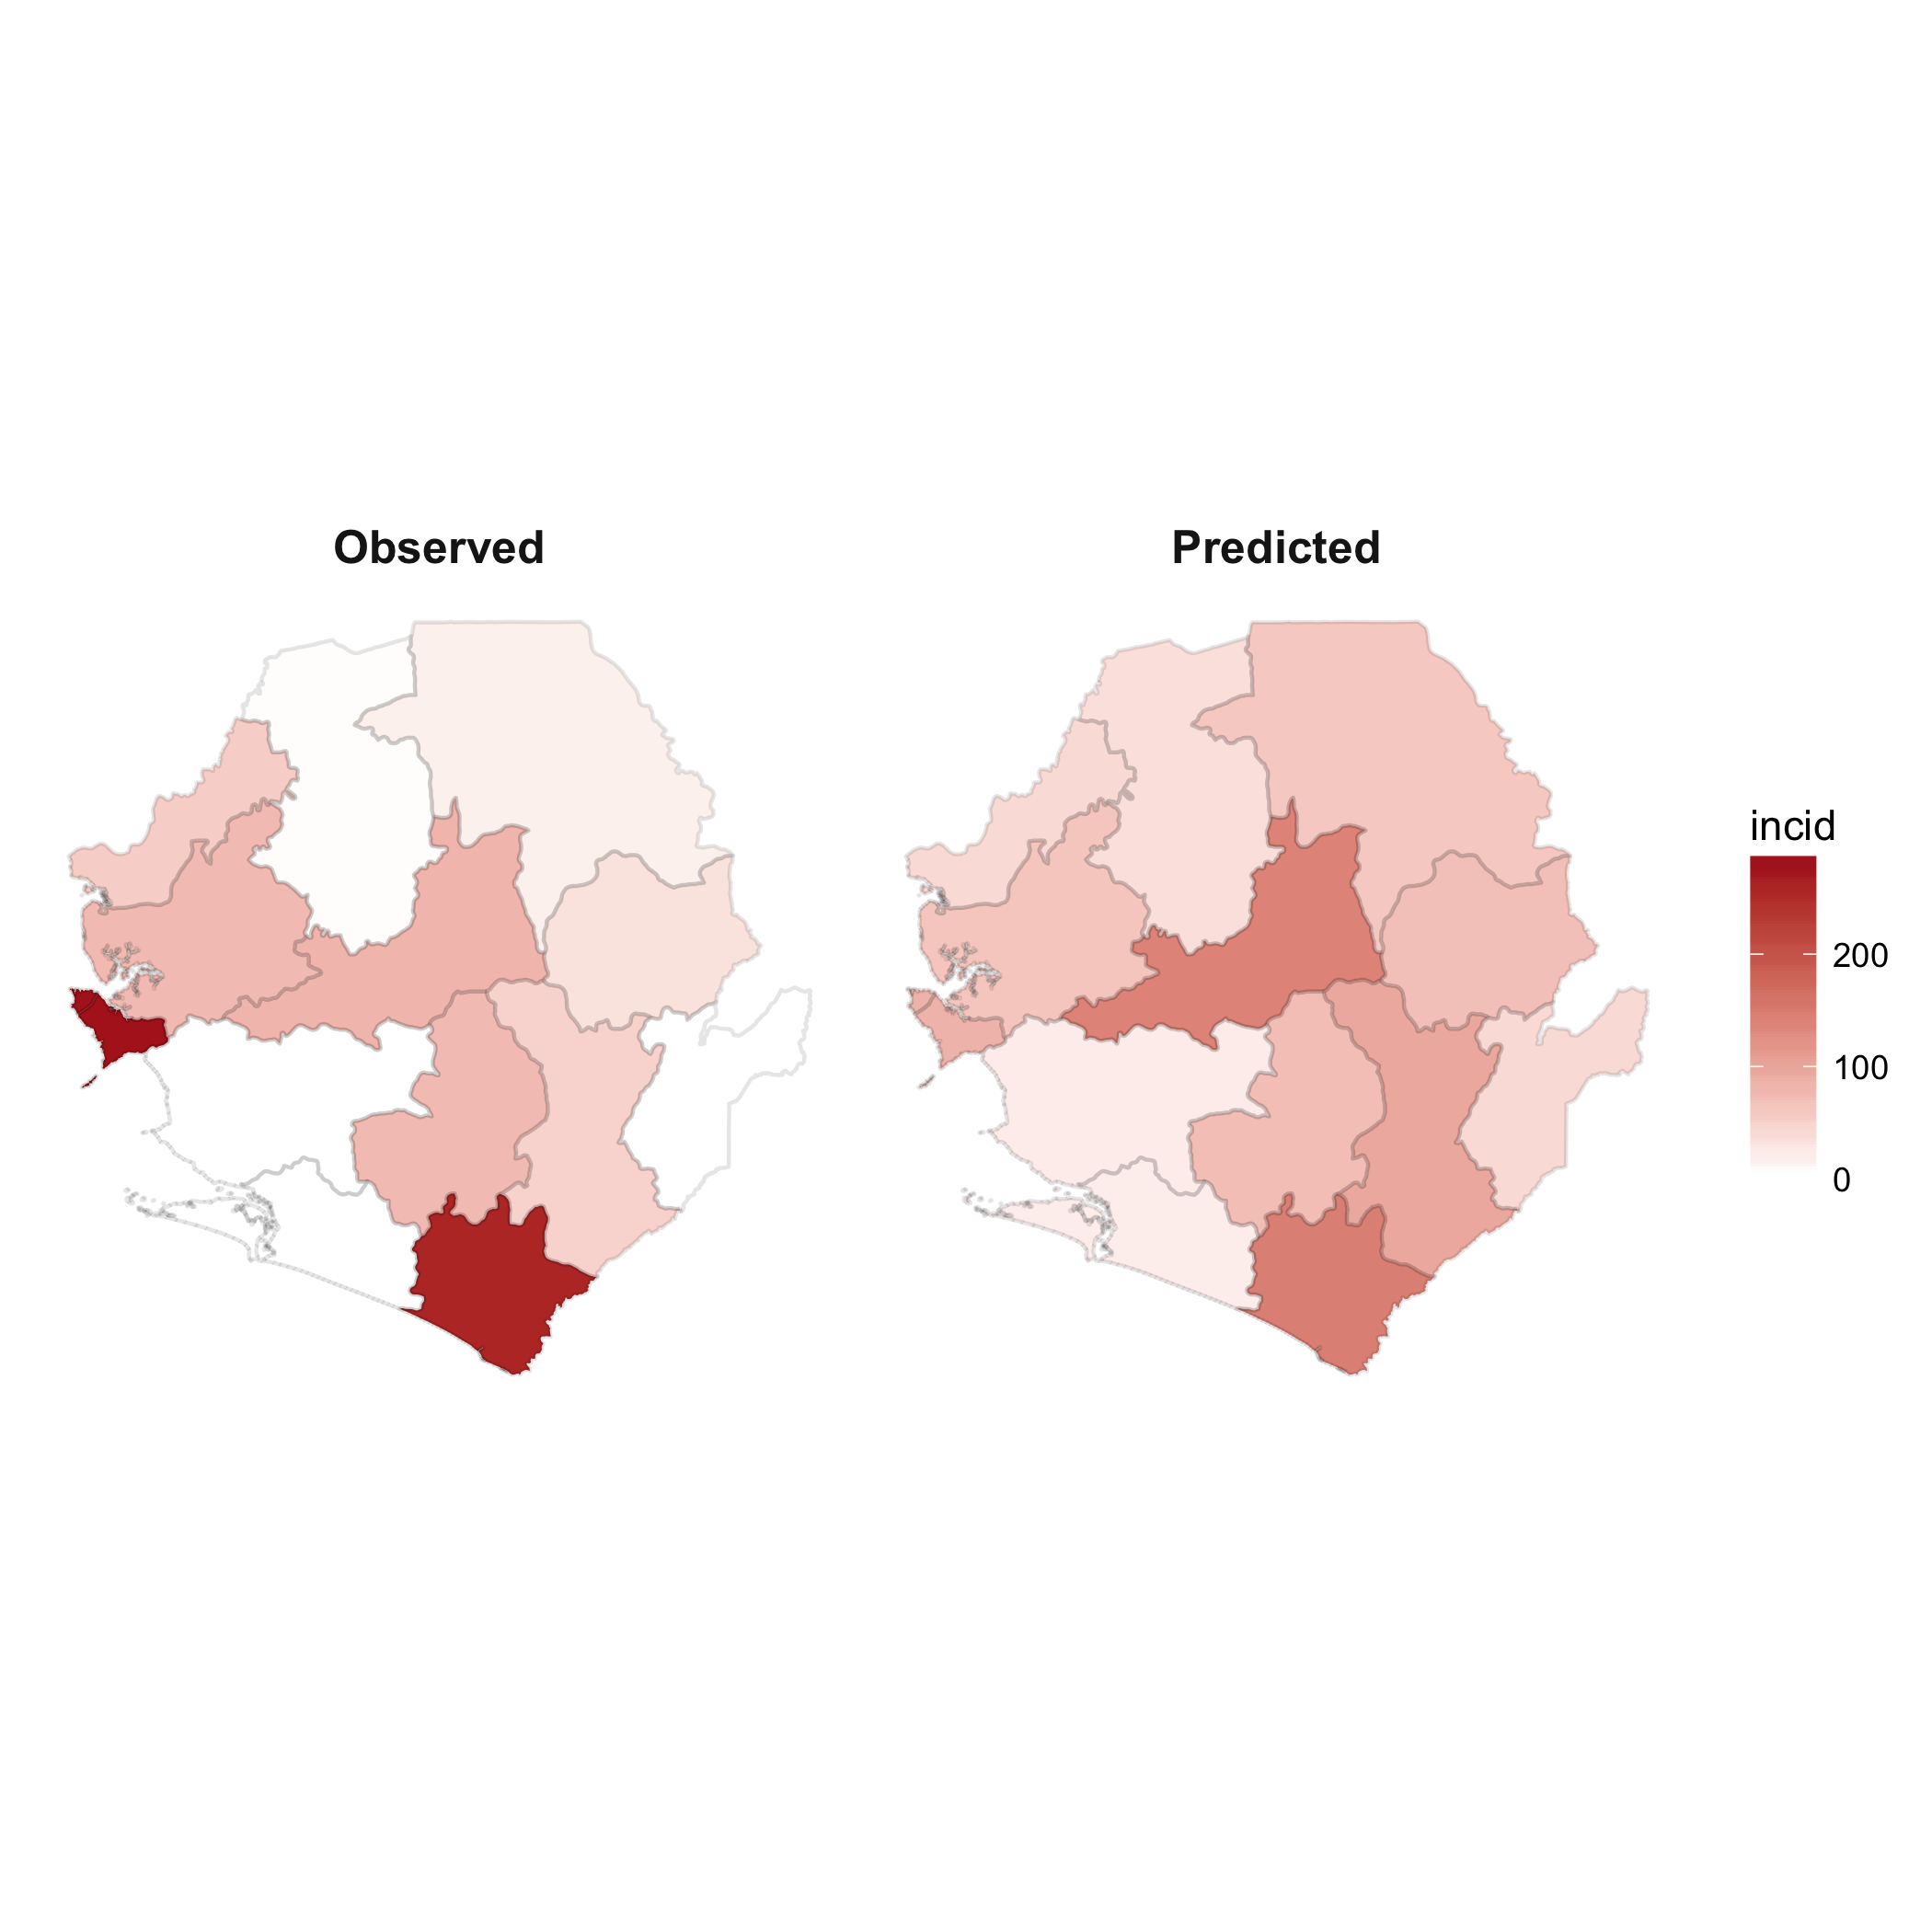
\includegraphics{ms6-figures/sl-map}
  \caption[Spatial spread of Ebola in Sierra Leone]{The map shows the
    observed (left) and predicted (right) spatial spread of Ebola in
    Sierra Leone over a 7 week period beginning in May 2015.}
  \label{fig:sl-map}
\end{figure}
\FloatBarrier

\section{Conclusions and next steps}\label{sec:conclusions}

The integration of the different data streams into the prediction
framework shows promising results in predicting the risk of spread of
an outbreak. The model was validated using both gross and
disaggregated data from the  2013 to 2016 outbreak of Ebola. The next
steps of this work include:

\begin{itemize}
\item estimation of parameters of the model including the influence of
  the health care capacity;
\item integrating the uncertainty in parameters in the prediction
  framework;
\item implement model selection and model averaging modules to account
  for model uncertainty as well.
\end{itemize}





\newpage

\bibliography{ms6}


\end{document}
